
\section{Introduction}

In this chapter, we will focus on the process scalable 12-bit 160 MS/s ADC designs, which mainly targets mobile long-distance communications such as 5G and 802.11ax WiFi SoCs \cite{kawai-11ax}.
Since such transceivers are most heavily used in mobile devices, the ADC's power efficiency is crucial to the device battery life.
While SAR ADCs becomes the priority design candidate when obtaining peak power efficiencies, SAR ADCs have the downside of reference settling, discussed in chapter 1.
Though it is possible to design such a high-speed and high-resolution SAR ADC, the overhead of peripheral circuits cannot be ignored; reference buffer may consume more power than the core ADC \cite{ccliu201612} or extremely large decoupling capacitors will be required.

Therefore, Pipelined-SAR ADCs become the most suitable architecture for such design targets.
By pipelining, the reference settling requirements of the SAR ADCs can be greatly relaxed and the overhead of peripheral circuits will be sufficiently small.
Moreover, by utilizing SAR ADC as the quantizer, high power efficiency can be expected.
However, to achieve high-resolution in Pipelined-SAR ADCs, high-accuracy residue amplification and high gain Opamps are required. 
As previously discussed, achieving high gain Opamps with scaled CMOS is a major design challenge.

\subsection{Review of conventional amplifiers for scaled CMOS designs.}

Realizing a suitable amplifier in scaled CMOS has been an active and important research area in the field of ADC designs.
For example, correlated level shifting (CLS) \cite{gregoire2008over} enhances the opamp gain by a square with two-step amplification. However, in deep-scaled CMOS, even square enhancement may be insufficient due to the degraded opamp gain. 

\begin{figure}[!]
\centering
  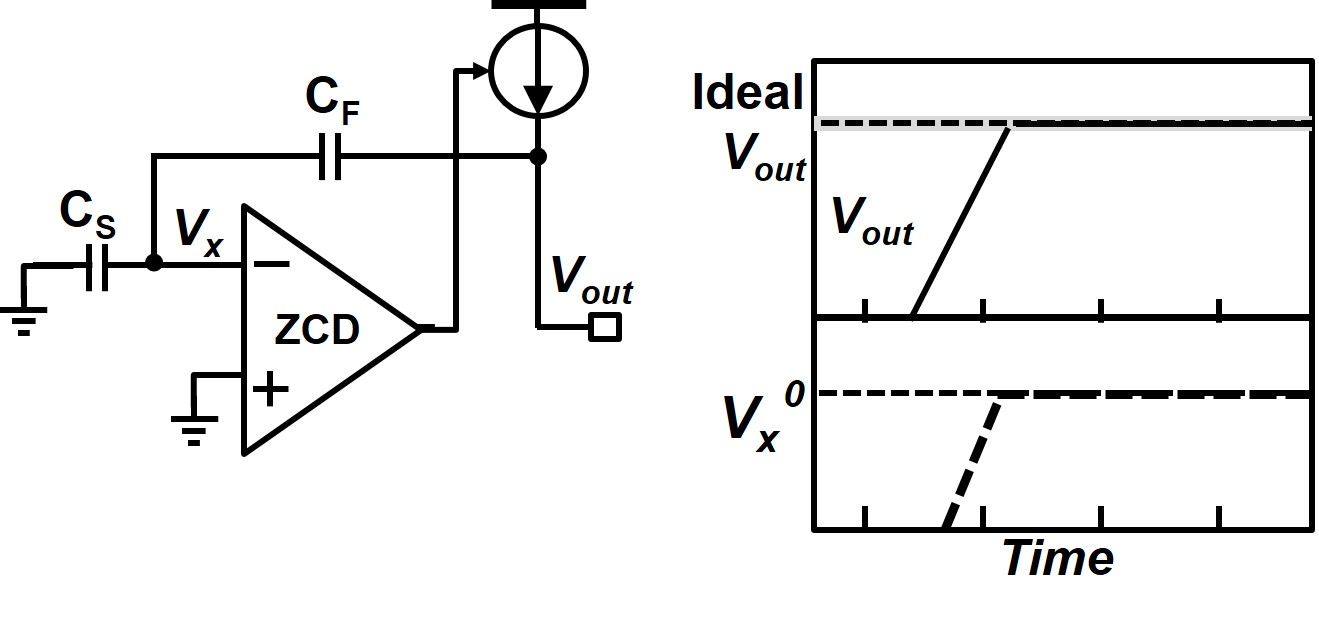
\includegraphics[width=1\textwidth]{figure/chap2/zcd.jpg}
  \caption{Zero crossing based amplifiers}
  \label{zcd}
\end{figure}

Zero-crossing-based amplifiers \cite{fiorenza2006comparator}\cite{zerocrossing}\cite{chang201411}\cite{brooks200912b} achieve efficient and accurate amplification by focusing on the virtual-ground node (Fig.\ref{zcd}. The amplifier output is charged by a current source and when the virtual-ground establishes a zero-voltage, the current source is cut off. The virtual-ground sensing can be realized by a simple zero-crossing-detector (ZCD). Ideally, this will achieve ideal amplification but several critical issues remain in real-life usages. Firstly, while the finite detection delay of ZCDs will become amplification offsets, such offsets may produce non-linearity reflecting the input voltage with low-output-resistance current sources. In scaled processes, improving the linearity of current sources is a big challenge since supply voltages are very low: e.g. cascading transistors are not available. 
Therefore, realizing high accuracy with ZCDs in scaled CMOS have similar challenges to the Opamp and is very difficult. Moreover, low-power ZCD designs are also challenging in high-speed converter designs because ZCDs are Opamps which draw large constant currents. Since the starved current scale with the amplification speed, realizing high power efficiency is challenging.

\begin{figure}[!]
\centering
  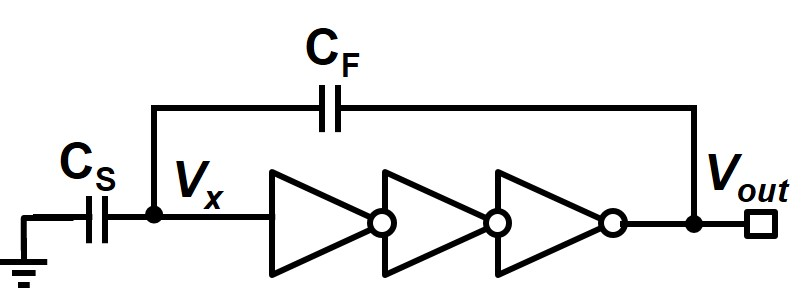
\includegraphics[width=0.9\textwidth]{figure/chap2/ring.jpg}
  \caption{Ring amplifiers}
  \label{ring}
\end{figure}

Finally, ring amplifiers \cite{hershberg2012ring}\cite{lim20151}\cite{hershberg2012phd} are also efficient amplifiers with emerging techniques. Ring amplifier operation differs from conventional amplification and there is a lot of room for new researches. 
Fundamentally, the ring amplifier gain is limited by the inverter gain, which degrades as the CMOS process scales.
The maximum achievable gain for a three-staged ring amplifier will be a cubic of a single inverter gain, which may be around 40-50dB in scaled CMOS process in the worst corners, and thus inefficient for high-accuracy pipelined converters. Most advanced ring amplifiers utilized in 16nm CMOS utilize digital calibration, though the proposed calibration itself is unique and quite inexpensive \cite{hershberg-ring-16nm} \cite{hershberg-ring-16nm2}.

\subsection{Shortcomings of digital gain calibration}

Hence, a number of designs utilize digital calibration to counter the gain error and to tolerate the use of low-gain amplifiers. Since precise gain is not required, this approach allows the use of efficient open-loop (or dynamic) amplifiers  \cite{murmann200312}\cite{verbruggen201470}\cite{zhou201512}\cite{verbruggen20132}. 
Since digital circuits lower its cost with process scaling, the calibration circuit cost becomes negligible as years pass by.
Then, why should we target "calibration-free" ADCs if digital calibration plays along well?

To answer that question, we must deeply analyze the shortcomings of digital gain calibration.
First of all, digital gain calibrations not only require digital circuits but also require non-negligible additional analog circuitry as well. Secondly, even with background calibrations, there are environmental drifts that cannot be canceled which must be suppressed by expensive analog circuitry.

While there are several approaches to digital gain calibrations, the most major type is the split-ADC calibration \cite{mcneill2005split1}.
Split-ADC converts the input signal using 2-sets of ADCs but adds perturbation to each ADC input. Similar to dithering, the gain calibration coefficient can be calculated from each ADC's output differences. While this method can track the environmental drifts, 2-sets of ADCs are required to achieve the same performance; doubling the ADC power and area.
A single ADC can be operated with different perturbations if the calibration is only run foreground. While this approach will save area, the ADC cannot track environment drifts. Moreover, to achieve high-accuracy, the calibration requires many ADC conversion data. Ref. \cite{digitalcalpipeline} indicates that $2^22$ of samples are required to achieve 12-bit linearity in a 14-stage pipelined ADC, meaning that such calibration will end up in lengthy SoC startup times.

Another simple way to calibrate the gain is to utilize an accurate DAC and input ideal signals to the ADC. If the input value is known, one can easily calibrate the ADC gain. The main challenge in this approach is that a DAC achieving higher accuracy than the ADC must be designed. If the ADC is effectively 10-bits, the DAC should perform more than effectively 12-bits, which is quite challenging in scaled CMOS, and such analog circuitry may consume high cost. 

Moreover, sudden supply voltage variations cannot be tracked by gain calibrations. Remember that power supply noise rejection correlates with the amplifier gain. Thus, low-gain opamps and open-loop amplifier's accuracy are severely damaged by power supply noise.
Such fluctuations must be suppressed by analog circuits: with bypass capacitors, or voltage buffers. However, large bypass capacitors significantly impact chip cost and voltage buffers are power-hungry.
\color{black}

\subsection{Our approach}
To establish a process scalable amplifier for Pipelined-SAR ADCs, we propose the digital amplifier (DA) technique. 
DA cancels out all errors of the low-gain amplifier by feedback based on successive approximation (SA). Errors are detected by judging the virtual ground polarity and canceled out by a C-DAC connected to the MDAC output. Unlike conventional amplification techniques, the amplification accuracy is determined by the C-DAC LSB step and decoupled from transistor intrinsic gain, which brings a new design paradigm for ADC designs in scaled CMOS process. 

The DA is used to realize a calibration-free 0.7V 12-bit 160MS/s pipelined-SAR ADC \cite{yoshioka201728} \cite{yoshioka-digitalamp-journal}. Without any calibration, the ADC achieves SNDR of 61.1dB and FoM=12.8fJ/conv., which is over 3$\times$ improvement compared with conventional calibration-free high-speed pipelined ADCs. Furthermore, the ADC area including bypass-capacitor is only 0.097mm$^2$. 

This chapter is constructed as follows: Section 2.2 describes the main concept and its amplification characteristics of the DA. Then, further analysis of the DA is done in Section 2.3. Section 2.4 discusses the designed pipelined-SAR ADC and circuit implementations are disclosed in Section 2.5. Finally, measurement results are discussed in Section 2.6, along with the inter-process comparison.


\section{Digital Amplifier}
\subsection{Review of Opamp based amplifications}

\begin{figure}
\centering
  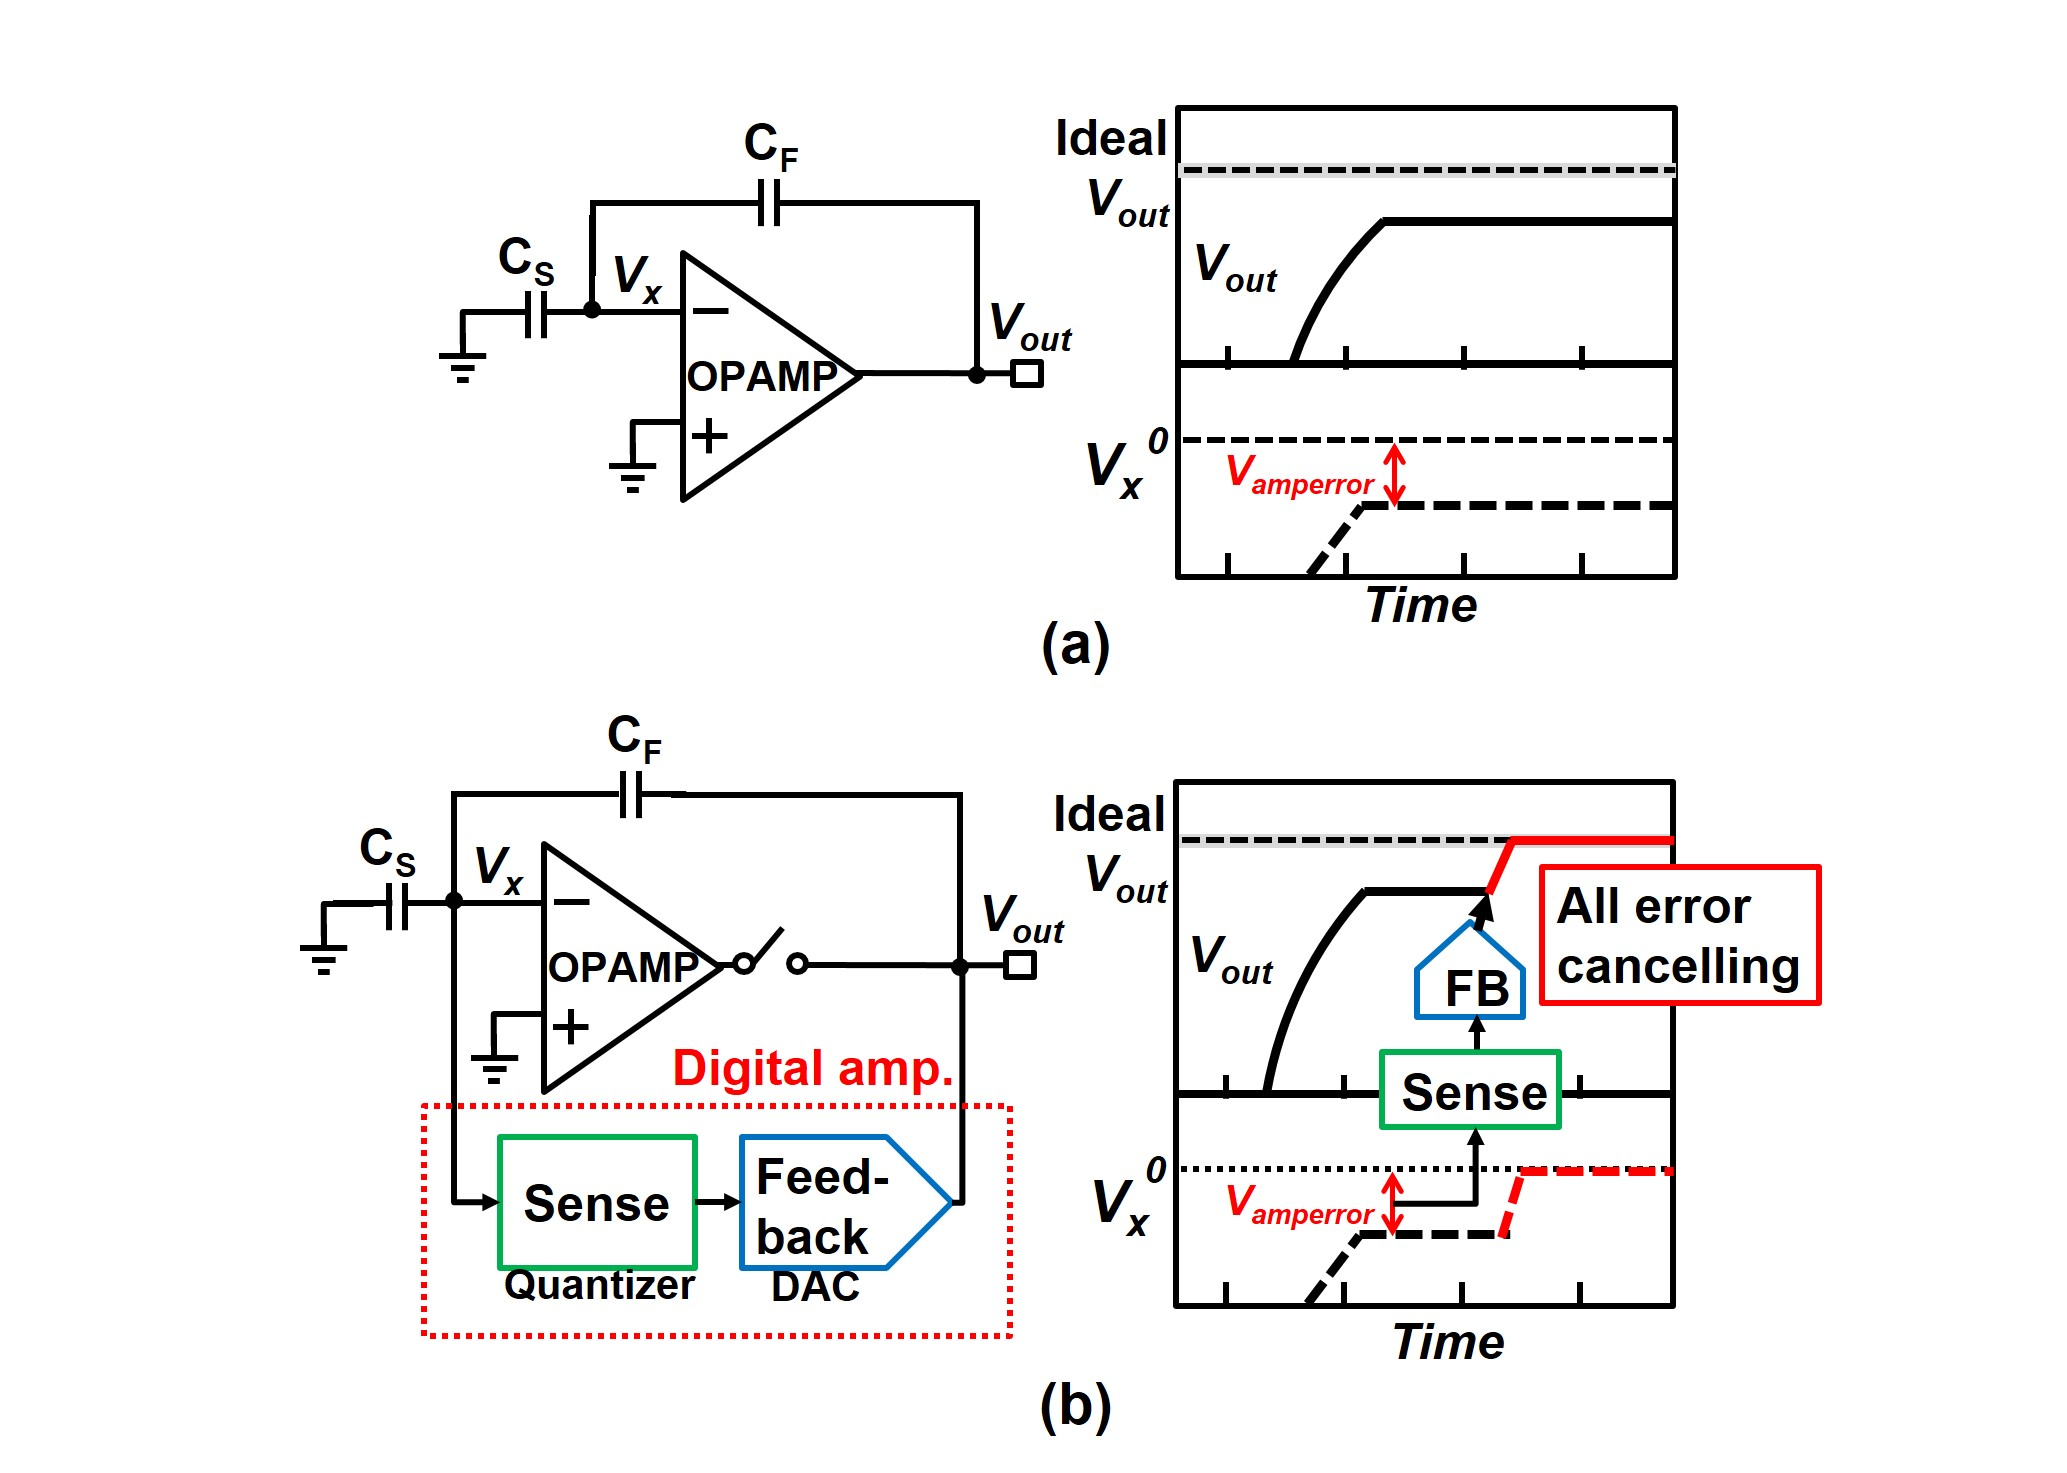
\includegraphics[width=1.1\textwidth]{figure/chap2/concept.jpg}
  \caption{(a) Amplification error due to the finite gain of opamps. A portion of the amplification error is observed at the virtual ground $V_x$. (b) Concept of the Digital Amplifier is shown. By \textit{directly sensing} the $V_x$ value and applying feedback to the output, digital amplifier cancels all opamp-induced-errors (finite-gain, incomplete settling, thermal noise, etc.).}
  \label{fig-concept}
\end{figure}

Before going to the details, we will start by studying an opamp-based switched-capacitor (SC) amplifier and examine its accuracy bottlenecks in scaled CMOS. 
If the opamp has an infinite gain, ideal amplification is done: the output voltage will be ideal ($V_{outideal}$) and virtual ground $V_x$ will converge to zero. On the other hand, with finite gain (Fig.\ref{fig-concept}(a)), an amplification error originating from the finite gain will occur. If the closed loop gain is  $A = A_{openloop} \times \beta$ ($\beta$ = feedback-factor):
\begin{eqnarray}
V_{out} &=& V_{outideal} \times \frac{A}{1+A} \\
V_{amperror} &=& V_{outideal} - V_{out} \approx \frac{V_{outideal}}{A}
\end{eqnarray}
Such amplification errors will cause harmonic distortions in pipelined ADCs, degrading the SNDR. To design a pipelined-SAR ADC achieving our design target (SNDR$>$60dB), system simulations imply that $A>$60dB will be required. Designing such amplifiers in scaled CMOS is very challenging; the achievable $A$ can be small as 20dB at worst conditions. 
 
 
\subsection{Digital Amplifier Principles}
%%%%%%
\begin{figure}
\centering
  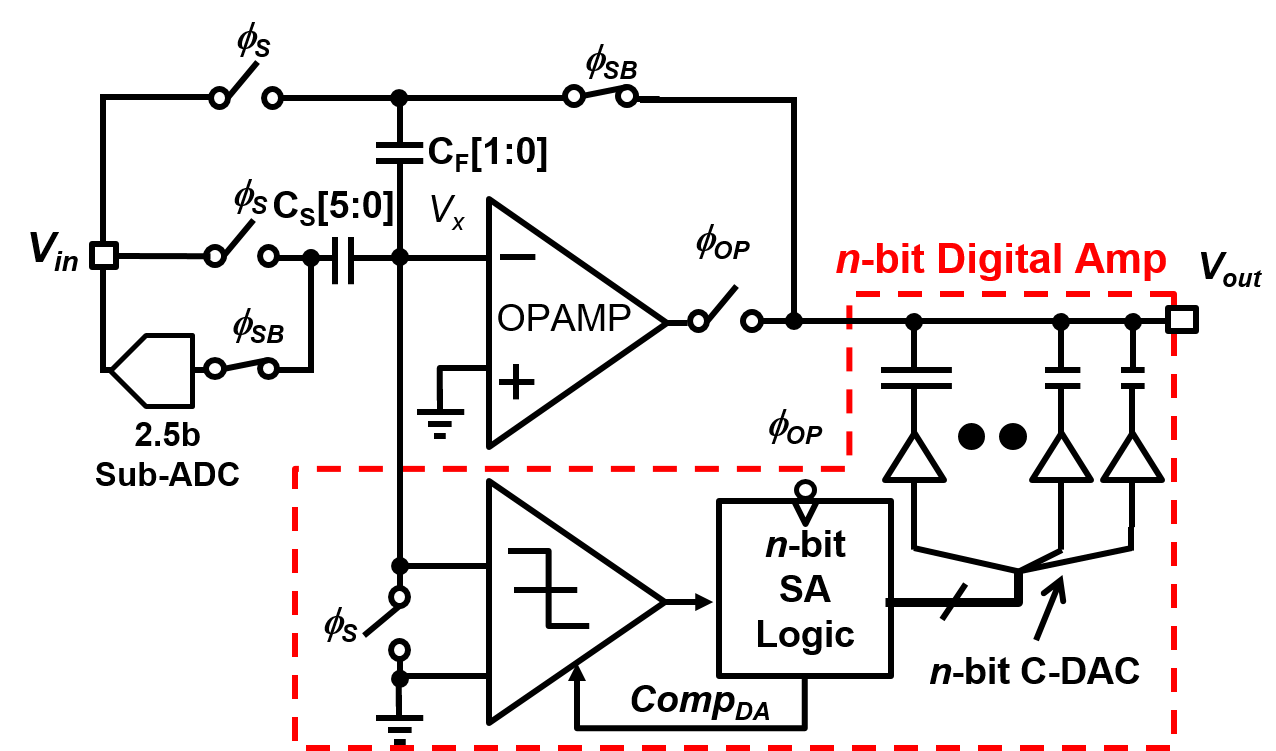
\includegraphics[width=0.9\textwidth]{figure/chap2/da-top.png}
  \caption{Schematic of a 2.5-bit flip-around MDAC with $n$ bit Digital Amplifier. }
  \label{fig-da-top}
\end{figure}
%%%%%%%

We propose the digital amplifier (DA) technique to realize an efficient and process-scaling SC amplifier.
DA cancels out all errors the opamp generates, which include gain error, non-linearity, incomplete settling, power supply noise, and thermal noise. In this section, we first study how the DA achieves a fine effective loop-gain. The main concept of the DA is shown in Fig.\ref{fig-concept}(b). DA operates with a 2-step amplification, where the opamp first performs a coarse amplification and then the DA cancels out the errors opamp produced. 
By \textit{directly sensing} the value of $V_x$ by a quantizer and canceling out the errors by feedback via DAC connected to the amplifier output, ideal amplification can be achieved by converging $V_x$ to zero. 

The amplification error of the opamp can be shown as below.
\begin{equation}
V_{x} = V_{amperror} \times \beta
\end{equation}
From above, we can derive the DAC transition ($V_{DAC}$) as:   
\begin{equation}
V_{DAC} = - \frac{V_{x}}{\beta} + N_{Q}
\end{equation}
\begin{equation}
V_{out} + V_{DAC} = V_{outideal} + N_{Q}
\end{equation}
Here, the amplification error $N_{Q}$ is the total quantization noise of the quantizer and the DAC. Interestingly, this implies that while conventional amplifiers' accuracy were limited by transistor intrinsic gain, the DA accuracy is only limited by the feedback circuit's quantization noise (or resolution). The feedback circuit resolution is a much easier parameter to configure than transistor gain in scaled processes. We will describe this point further in later sections. 

%The fundamental concept of the DA is similar to ZCB amplifiers\cite{zerocrossing}, where the amplification error is sensed via the virtual ground and $V_{out}$ is controlled to cancel that out. However, since ZCB utilizes analog comparators and current sources to realize the amplification (in terms of continuous value and time), their performance can be degraded with scaled CMOS integration. Therefore, we target a "digital" implementation (discrete-time and quantization) to maximize the process scalability of the amplifier.

\subsection{Digital Amplifier Implementation}

%%%%%%%%%%%
\begin{figure*}[!]
\centering
  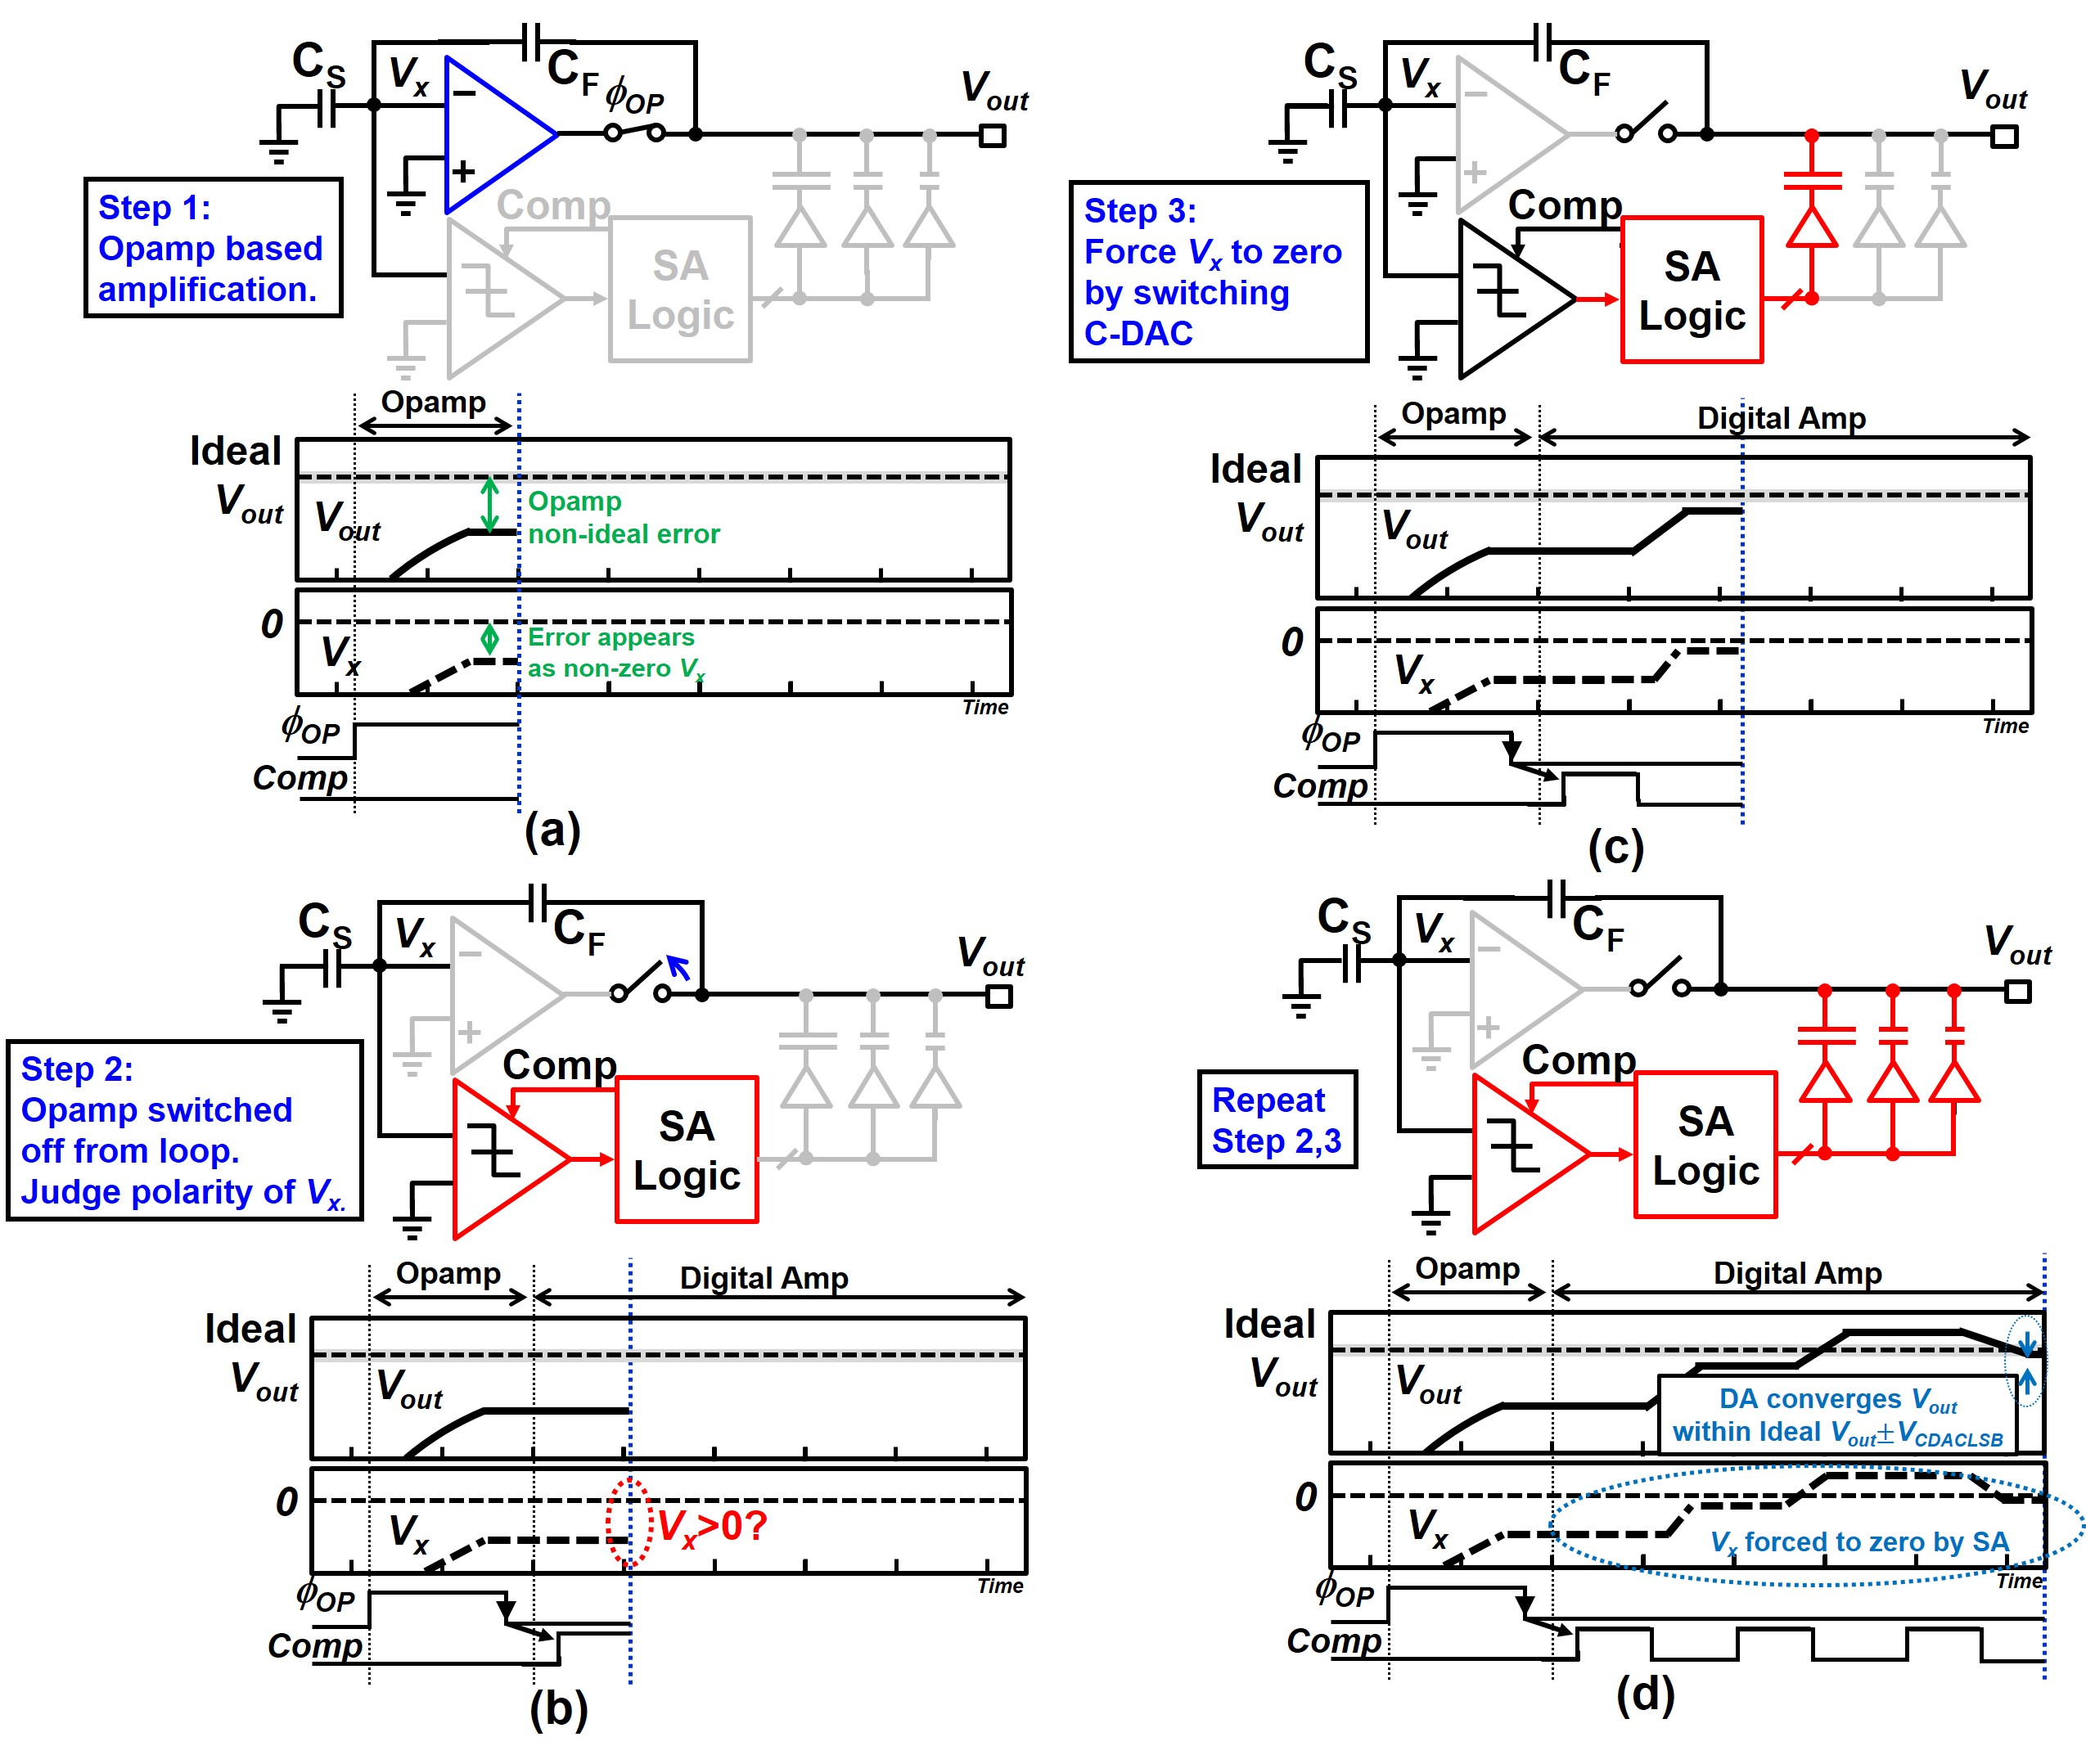
\includegraphics[width=1\textwidth]{figure/chap2/da-operation.jpg}
  \caption{Operation of the Digital Amplifier broken down in 4 steps. For simplicity, the DA is shown a 3-bit but the actual design is 8-bit.}
  \label{fig-da-operation}
\end{figure*}
%%%%%%%%%%%

To implement our proposed DA concept, a multi-bit quantizer and DAC will be required. Several requirements are: 1) fast so that it will not limit the amplifier speed (few $ns$) 2) minimum cost (area and power).
To satisfy the two requirements, we propose a successive approximation (SA) inspired implementation of the DA (Fig.\ref{fig-da-top}). Since SA requires only a single-bit comparator, SA-logic, and C-DAC, the implementation cost is low. Moreover, SA conversions are very fast in scaled processes \cite{kullsar} and the amplifier speed is likely not to be limited by DA.  

Here, the operation of the DA-based MDAC is explained step-by-step.
As quoted previously, the MDAC operation is split into 2 phases: opamp and DA.
During the opamp phase (Fig.\ref{fig-da-operation}(a)), $\phi$OP rises and the low-gain opamp is connected to the MDAC output to perform amplification. However, an error occurs owing to the non-ideal effects of the opamp.  
$\phi$OP is driven by a 2ns long pulse and when $\phi$OP sets down, the opamp is cut off from the loop and DA is activated (Fig.\ref{fig-da-operation}(b)). 
During the DA phase, the virtual ground is forced to zero by carrying out feedback based on successive approximation (SA), utilizing a clocked comparator and a C-DAC. The comparator judges the polarity of $V_x$ (Fig.\ref{fig-da-operation}(c)) and the C-DAC connected at the MDAC output is controlled so that $V_x$ will converge to zero. The SA operation is repeated for $n$ cycles; $V_{out}$ will always converge to the ideal $V_{out}$ with an error range of the C-DAC LSB voltage ($V_{CDACLSB}$), which also stands for the amplification error in DA (Fig.\ref{fig-da-operation} (d)). Note that while the DA generates digital codes to configure the C-DAC, this code is only used for amplification and not used for the final ADC output.

By configuring the number of bits in SA, the DA can arbitrary coordinate its amplification accuracy. However, the drawback is as the number of bits increases, the number of SA cycle during the amplification increase as well. Therefore, similar to a SAR ADC, a tradeoff exists between the amplification time and amplification accuracy in DA. To achieve higher accuracy with constant amplification time, speed-enhancing techniques such as 2-bit/step \cite{cao200832mw}\cite{yoshioka20158} can be adopted but will impact the power and area.

\section{Further Analysis of Digital Amplifier}
\subsection{Amplification Error Characteristics}
In this section, the DA amplification error characteristics are analyzed for deeper understanding.
A significant feature of the DA is that its gain error is determined by the step size of $V_{CDACLSB}$ and is irrelevant to intrinsic gain.  $V_{CDACLSB}$ can be easily halved by increasing the DA resolution by 1-bit, which is equivalent to improving the opamp loop-gain by 6dB.
In this analysis, we will assume that the DA C-DAC output range is equal to the maximum error the opamp will generate. 
The DA's effective gain principal can be shown as below, assuming that DA's effective loop gain is $A_{DA}$, opamp loop gain is $A_{op}$ and DA number of bit as $n$: 
\begin{equation}
\label{eq:eq-gain}
A_{DA} = A_{OP}+6 \times n
\end{equation}

For further understanding, we will show a specific design example of our MDAC.
Our opamp designed in 28nm CMOS can achieve only 20dB loop-gain with the worst conditions, contrary to $>$60dB loop-gain required for the ADC target performance. From Eq.\ref{eq:eq-gain}, by designing a 7-bit DA, the amplifier loop-gain is boosted to: 
\begin{equation}
    20 \text{dB}+6 \text{dB} \times 7\text{bit}=62 \text{dB}
\end{equation}
and the design requirement can be easily met. As a result, over a cubic enhancement of $A_{OP}$ is achieved with DA, while techniques such as CLS are limited to a square \cite{gregoire2008over}. Interestingly, since the gain-error is mostly determined by the step size of $V_{CDACLSB}$, it is quite robust to PVT variations. %once the system is designed with the worst opamp gain. 
DA can greatly save design time because little tuning is required while iterating through PVT and post-layout simulations (contrastive to conventional opamp designs which require extensive design efforts, where the transistor characteristics vary widely through PVT and layout).

\subsection{Power Optimization Strategy}
%%%%%%%%%%%
\begin{table}[!]
\centering
  \caption{Normalized settling error requirements for opamp and DA based MDACs, respectively.}
  \label{tbl:da-vs-op}
  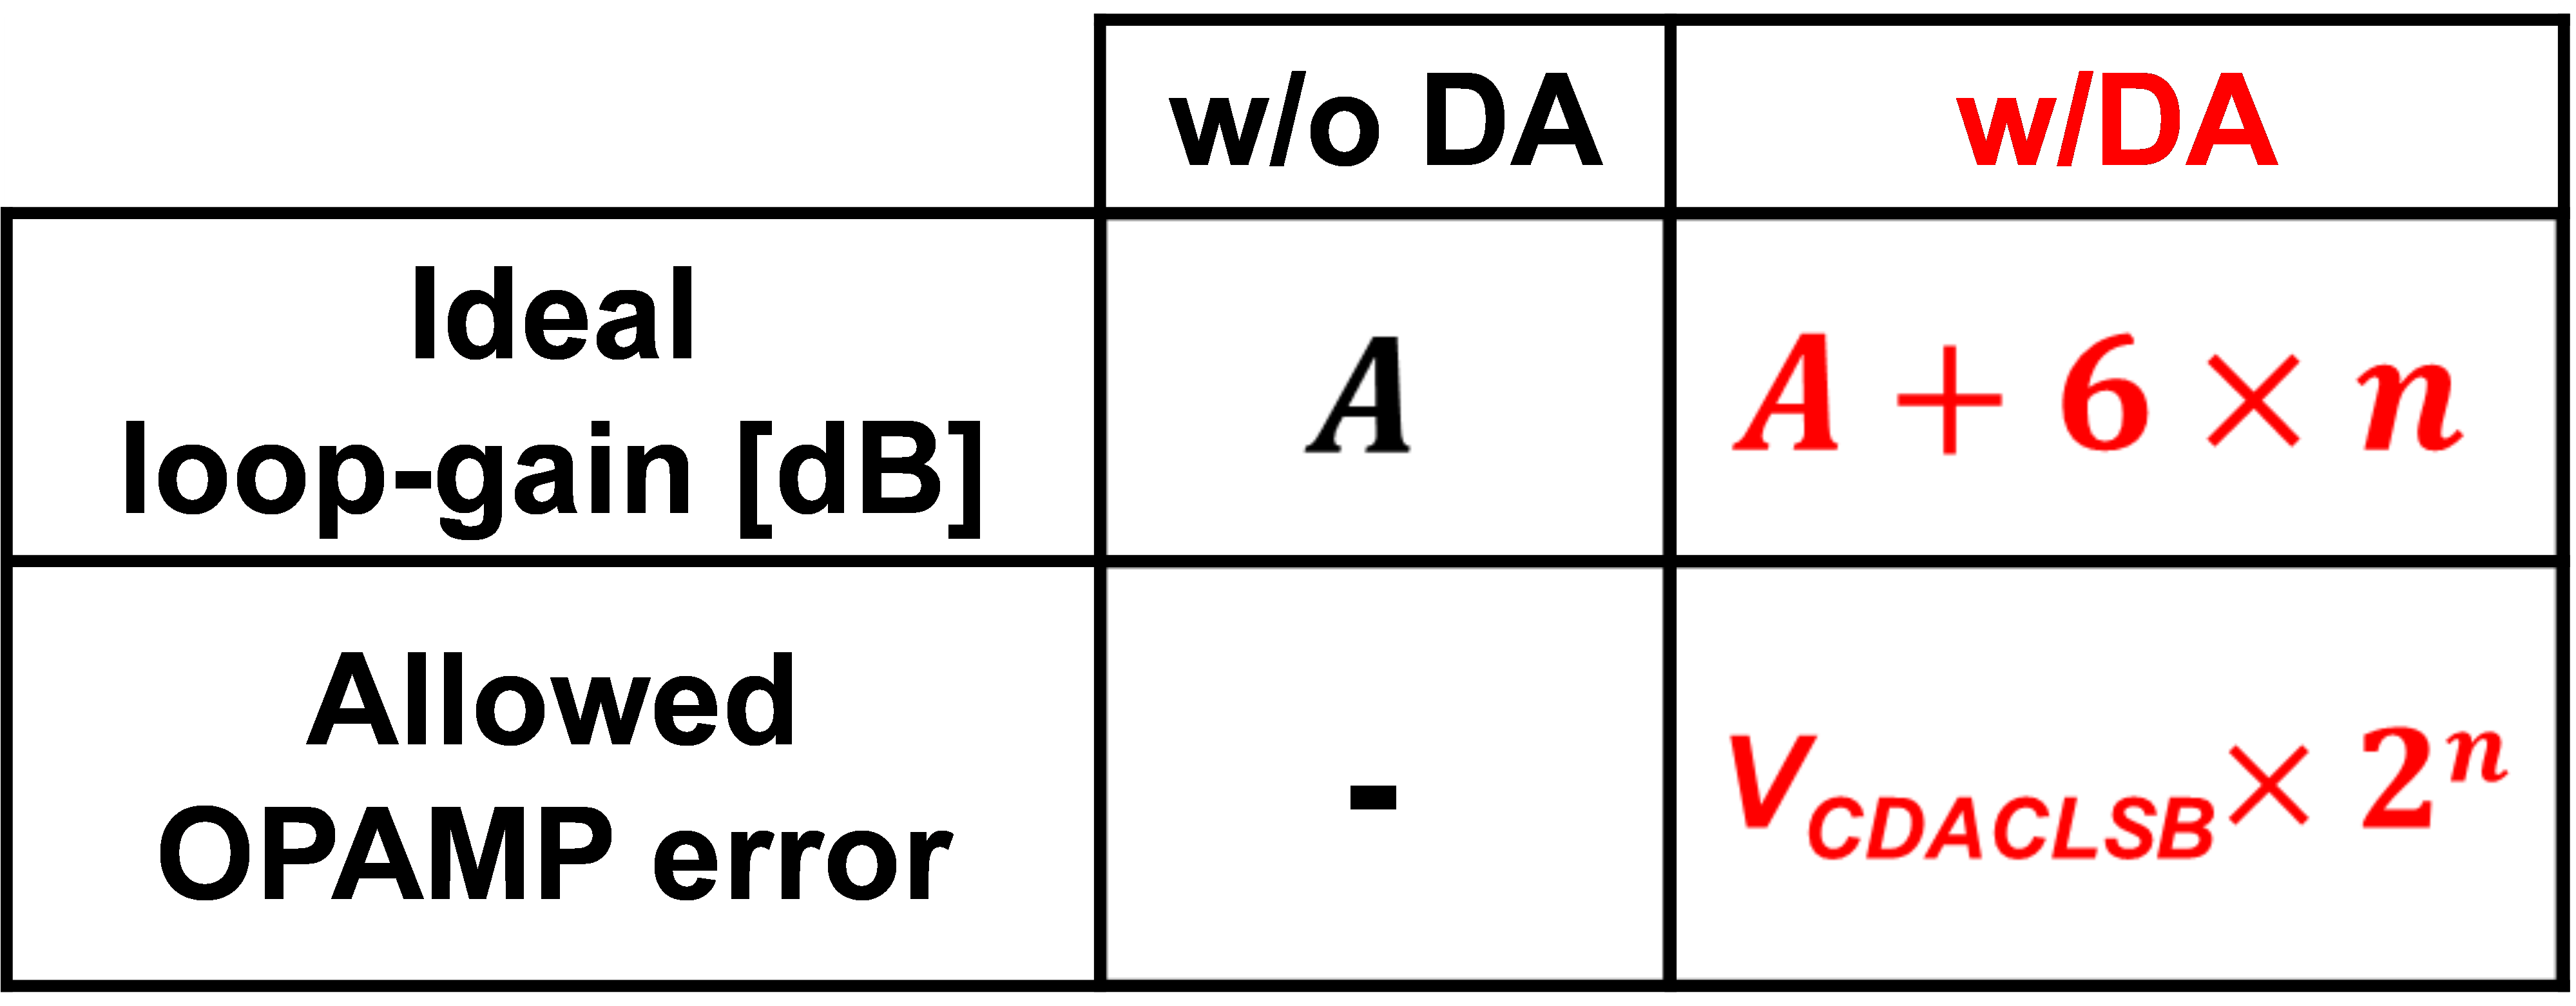
\includegraphics[width=0.7\textwidth]{figure/chap2/amp-chara.png}
\end{table}

\begin{figure}[!]
\centering
  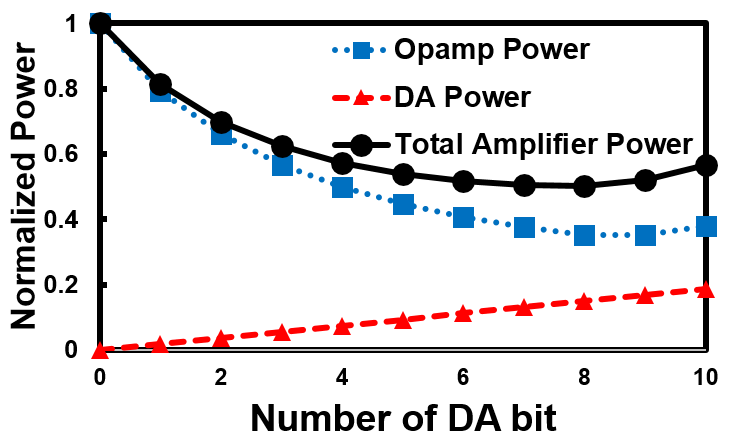
\includegraphics[width=0.9\textwidth]{figure/chap2/da-vs-opamp.png}
  \caption{Number of DA bit versus estimated MDAC power is plotted. 0-bit case is a MDAC designed only with an opamp. MDAC power starts to increase after DA's settling error mitigation effect saturates at a certain point.}
  \label{fig-amp-chara2}
\end{figure}
%%%%%%%%%%%
%%%%%%%%%%%
\begin{figure}[!]
\centering
  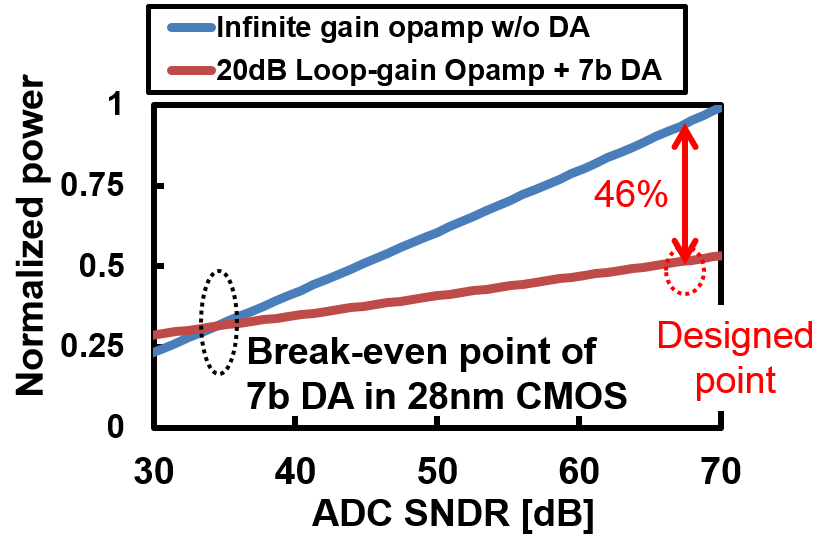
\includegraphics[width=0.9\textwidth]{figure/chap2/power-vs-sndr-analysis.png}
  \caption{
  We compare the power consumption of opamp-based and DA-based MDAC, respectively. Since DA-based MDACs has a relaxed settling requirements, at DA=7-bit, 46\% power savings can be expected at our target SNDR design point.}
  \label{fig-power-sndr-analysis}
\end{figure}
%%%%%%%%%%%

In conventional high-speed pipelined ADC designs, the opamp must be designed with a strict settling error requirements, which easily overgrows the amplifier power consumption \cite{chai20125}. To obtain faster settlings, high Gain Bandwidth (GBW) is required, which is typically obtained by burning more power. 
In this section, we will discuss the DA-based MDAC power consumption assuming that the amplifier power is determined by settling requirements. We will show that by utilizing DA, significant power savings can be achieved compared to opamp-based designs because DA allows opamp designs with significantly relaxed settling requirements.

DA not only removes the opamp gain-related errors but can remove settling errors as well. Here, we will consider a 2.5-bit MDAC design with a settling error requirement achieving SNDR=66dB.   
According to ref.\cite{demerow1970settling}, the opamp settling error and GBW relationship can be shown as bellow. 
\begin{equation}
 \text{Settling req.} \approx \exp(-GBW)
\end{equation}
From the above, we can derive the relationship between the amplifier settling requirements and the required GBW (Table \ref{tbl:da-vs-op}). As shown in the table, utilizing an $n$-bit DA can relax the opamp settling requirements by $2^n \times$. However, since SA cycles must also be completed within the same amplification window, the effective time for opamp amplification will decrease with the increased DA bit. The \textit{effective} settling requirement can be derived as bellow.
\begin{eqnarray}
    Ratio &=& 1 - n \times t_{DA} \\
    \text{Eff.Settling} &=& \text{Settling req.} \times Ratio
\end{eqnarray}
Here, $t_{DA}$ is the normalized time for a single SA cycle. The effective settling requirements saturate around DA=8bit due to the fixed amplification time window. We will also estimate the MDAC power consumption, derived from the opamp GBW. The GBW can be expressed with $g_m$:
\begin{equation}
    GBW = \frac{g_m \times \beta}{2 \pi C_L}
\end{equation}
To simplify the analysis, we will assume constant current density, where doubling the $g_m$ will also double the power consumption. The opamp and DA's power consumption were derived from the 28nm CMOS post-layout simulation results and the power was scaled in respect to the required $g_m$ and bits. In Fig.\ref{fig-amp-chara2} we plot the MDAC power consumption against DA bits, where the power is normalized to the 0-bit case (MDAC designed only with an opamp). Since the DA's power is mainly dominated by the comparator and the SA-logic, the power increases almost linearly against the DA bit.
Increasing the DA bit relax the opamp settling requirements, thereby saving power.  However, since the effective settling requirement saturates around DA=8-bit, power savings also saturate around this point. Increasing the DA bit further than 8-bit has no effect and may even increase the power consumption.
Reflecting the results of this analysis, the DA bit is set to 7-bit in our design. While we fix the target SNDR to 60dB in our optimization strategy, the design point will change with higher target SNDR. Note that the comparator power increases 4$\times$ when the target SNDR rise 6dB. Thus for higher target SNDR, the power will be optimized with fewer DA bit.

Also, we conduct an analysis based on the target ADC SNDR versus MDAC power in Fig.\ref{fig-power-sndr-analysis}. Since settling requirements become strict with higher resolution, DA enjoys further power savings at high SNDR as well. At our design point of SNDR=66dB, the DA-based MDAC can save 46\% power compared to opamp-based designs.

%%%%%%%%%%%%%%%%%%%%%%%%%%%%%%%%%%%%%%%%%%%%%%%%%%%%%%%%%%%%%%
\subsection{DA's opamp noise-canceling feature}
We will show that the DA cancels out not only the gain error but the thermal noise of the opamp as well. While there will be opamp thermal noise present during the initial opamp-based amplification when the opamp amplification ends, the opamp is cut-off from the loop and its noise is sampled  (Fig.\ref{fig-da-operation}(b)). Since the opamp noise will simply appear at the $V_x$ node as amplification error as in eq. (3), the error is treated similarly as gain errors and settling errors;
DA will sufficiently cancel this out by successive approximation.

\begin{figure}[!]
\centering
  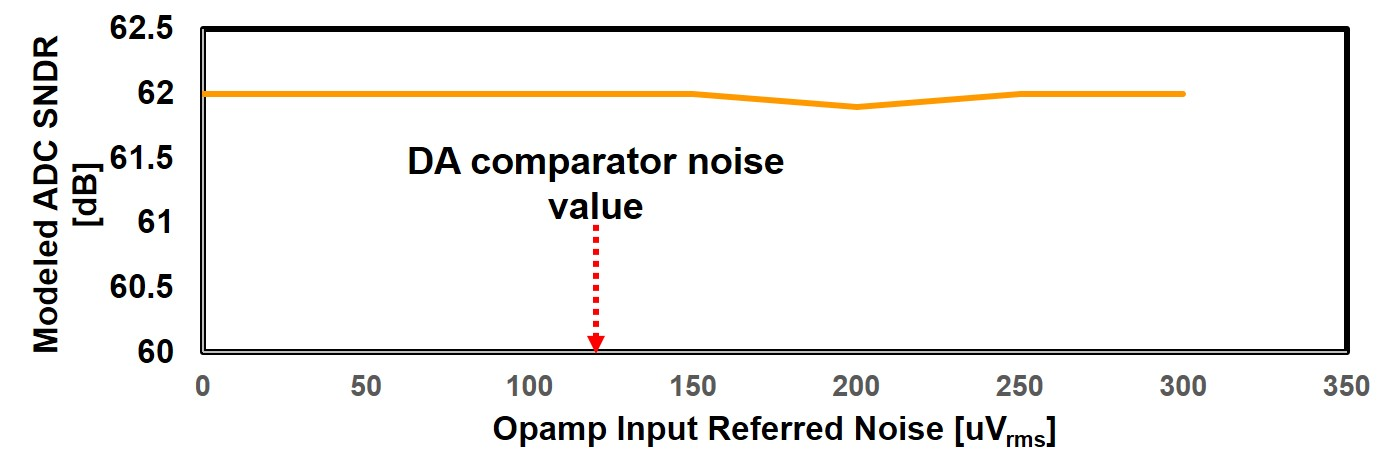
\includegraphics[width=1\textwidth]{figure/chap2/opamp-noise.jpg}
  \caption{The Matlab simulation results of the Pipelined-SAR ADC SNDR is shown, where the opamp noise is varied. }
  \label{fig-noise-opamp}
\end{figure}

Fig. \ref{fig-noise-opamp} shows the Matlab simulation results with varied opamp noise.
All of the other noise sources (sampling kT/C, DA comparator noise, etc.) are kept constant which uses the design values.
Interestingly, even if the opamp noise is varied for a large scale, it does not affect the overall ADC SNDR at all.
We can state that the DA "cancels" the opamp noise if the opamp noise is larger than that of the DA (the designed DA comparator noise is about 120uVrms). However, even if the opamp noise is better than that of the DA comparator noise, the overall amplifier output noise will be determined by the DA comparator noise. Therefore, in DA based designs, we must carefully design the comparator noise since it will largely dominate the ADC noise.
To note, in our design, the noise ratio between the opamp and the comparator was about the same amount.

\color{black}
%%%%%%%%%%%%%%%%%%%%%%%%%%%%%%%%%%%%%%%%%%%%%%%%%%%%%%%%%%%%%%

\subsection{Spurious-free Characteristics of the DA}
%%%%%%%%%%%
\begin{figure}[!]
\centering
  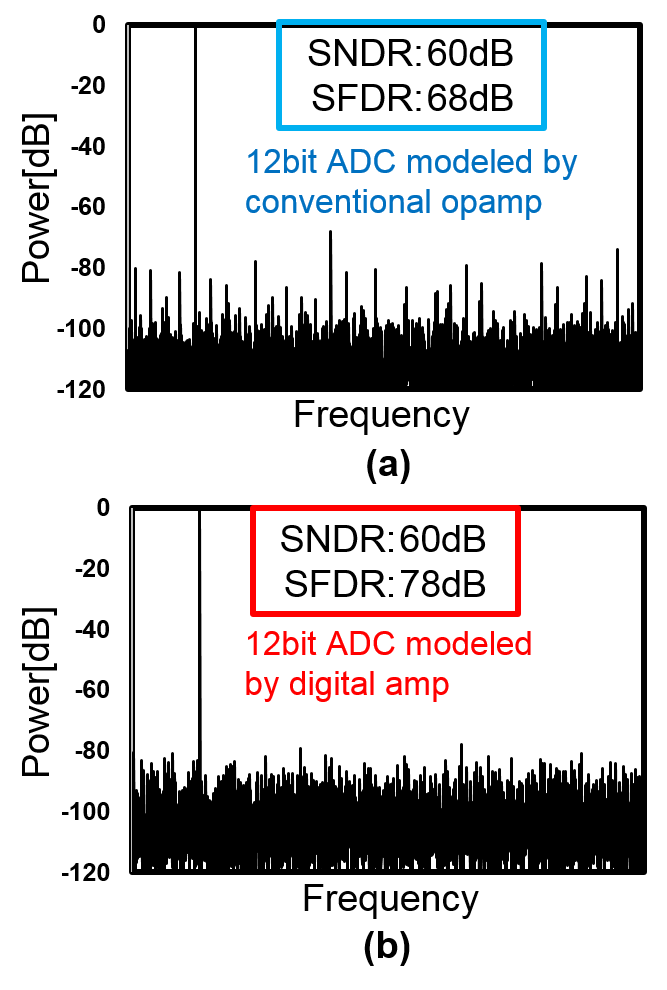
\includegraphics[width=0.8\textwidth]{figure/chap2/spur.png}
  \caption{Matlab simulated FFT results of the pipelined-SAR ADC are shown, where (a) uses opamp-based MDAC and (b) utilize DA-based MDAC. Since DA's gain error does not have correlation with the input signal, the SFDR excels by 10dB. Note that the opamp gain and DA bit were tuned to achieve the same SNDR. }
  \label{fig-spur}
\end{figure}
%%%%%%%%%%%

Another important feature of the DA is that fundamentally, the amplification is spurious-free.
Fig.\ref{fig-spur} compares the system simulation results of the pipelined-SAR ADC utilizing opamp-based and DA-based MDAC, respectively. The opamp amplification error can be derived from Eq. (1),(2) by:
\begin{equation}
    V_{amperror} \approx \frac{V_{in}}{\beta \times A}
\end{equation}
The error is a function of the input signal $V_{in}$. Since such errors will appear at the ADC spectrum as harmonic tones, the SFDR degrades  (Fig.\ref{fig-spur}(a)). The performance of wireless systems utilizing sub-carriers (e.g. OFDM) may degrade by such spurious tones and higher SFDR is preferred by the system. 

On the other hand, since the DA amplification error is quantization noise, the errors can be modeled as random values. Since the amplification errors appear at the noise floor, the SFDR excels compared to opamp-based implementations (Fig.\ref{fig-spur}(b)).
However, note that when the target SNDR is low, the DA quantization error gets correlation with the signal and may get worsened SFDR performances. If the target SNDR is high enough, as in this design (SNDR$>$60dB), the spurs will spread nearly to the noise-floor level and the ADC can achieve an enhanced SFDR performance. 
\subsection{Designing the SA range}
%% DAの設計方針などについて記述する。
Designing the SA range (or the C-DAC output range) of the DA is an important design topic and is deeply analyzed.
If the opamp generates error larger than the SA range, the DA cannot fully correct the amplification error and the amplification accuracy will be corrupted.
While this can be evaded by designing the SA range with large redundancies, it will require more DA bits to achieve the same precision and will slow down the amplification speed.
Therefore, the SA range should be the necessary minimum to minimize the DA overheads. 

How can we estimate the necessary minimum amount of the SA range?
To be specific, the majority of the opamp error can be broken down as follows: 1) error due to opamp infinite gain, 2) error due to opamp incomplete settling.
While there are other sources such as opamp error due to thermal and power supply noise, such noise is small compared to the former errors and can be neglected.
During the design, we should estimate the total error with simulations. One way to conduct this is by applying the switched capacitor amplifier several input patterns and comparing the output against the ideal output. Therefore, we can obtain the generated opamp error for each test case. By conducting this simulation with various PVT settings, we can obtain the maximum error the opamp generates.
Using these results, we can define the required SA range for one's design.

\section{Pipelined-SAR ADC Architecture}
% アーキテクチャ
\begin{figure*}[ht!]
\centering
  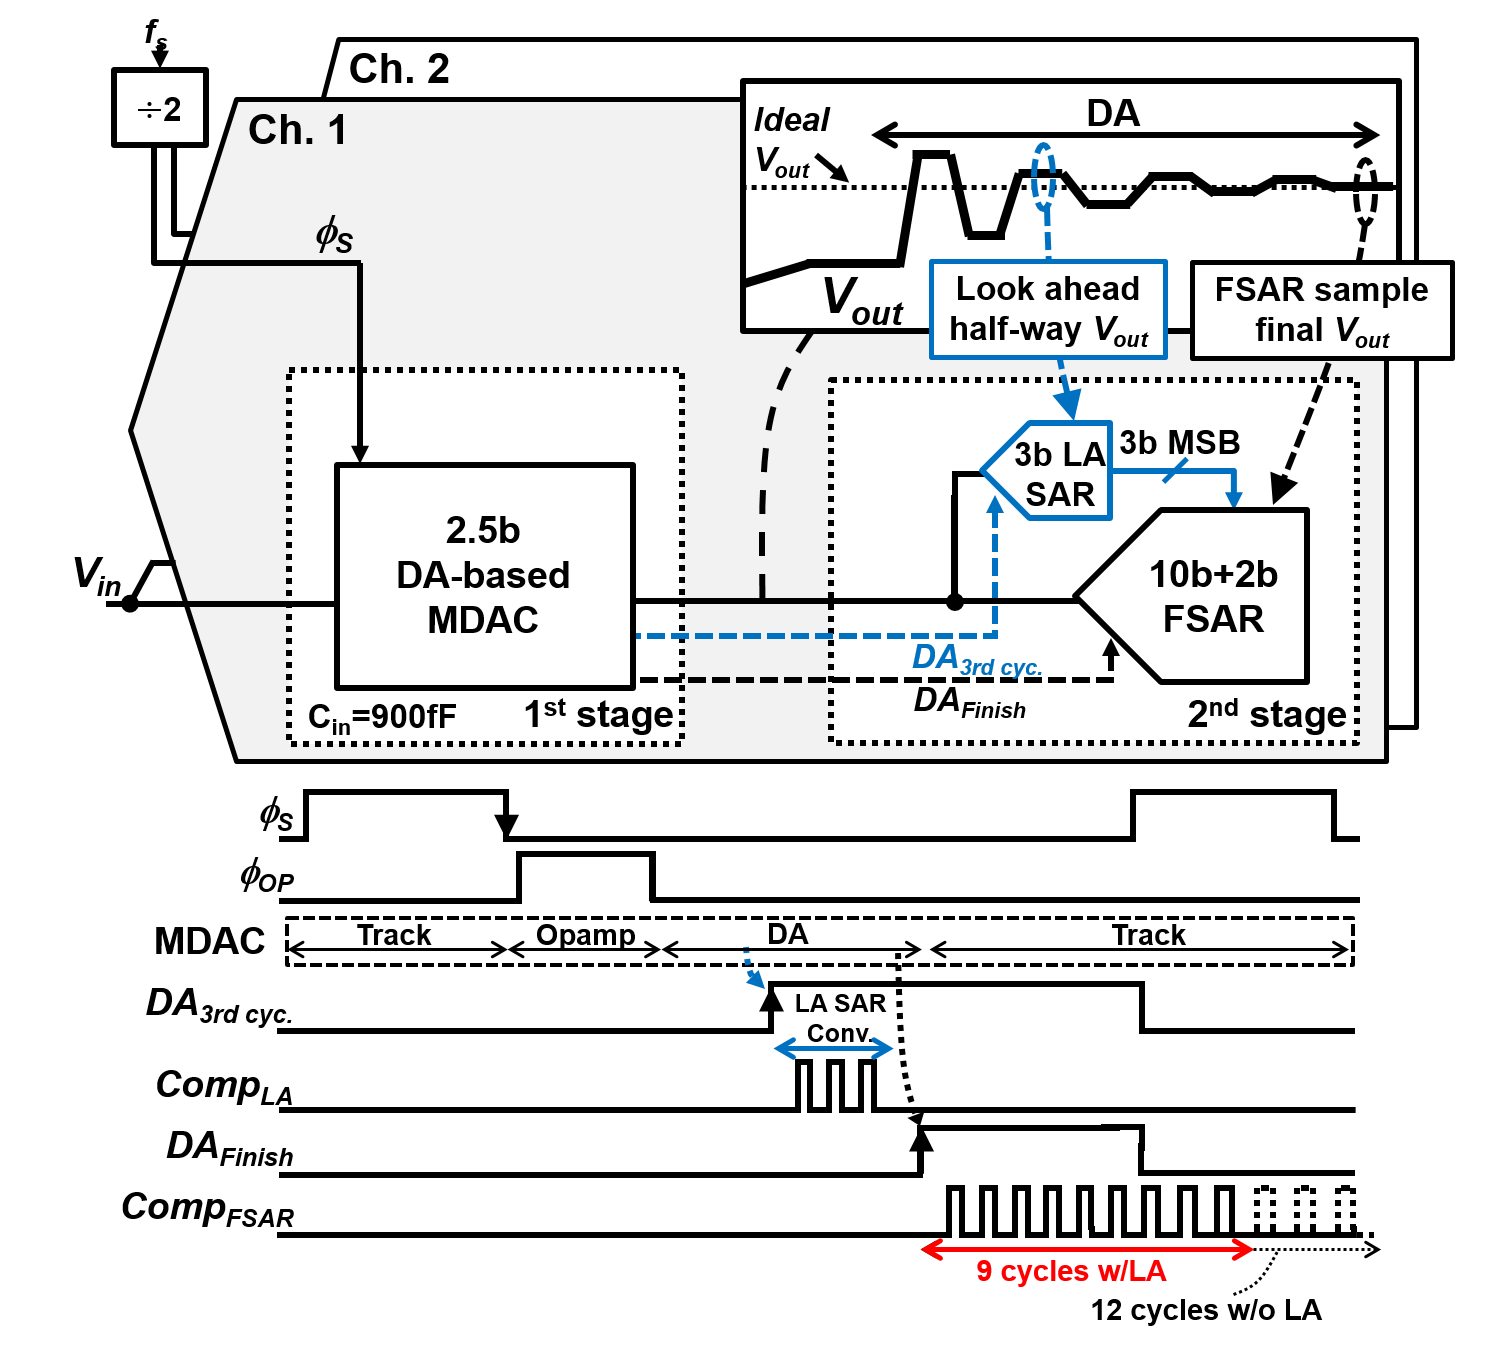
\includegraphics[width=1\textwidth]{figure/chap2/architecture.png}
  \caption{The architecture of the two-way interleaved 12bit 160MS/s pipelined SAR ADC.}
  \label{fig-overview}
\end{figure*}


Fig.\ref{fig-overview} shows the block diagram and timing chart of the two-way interleaved pipelined-SAR ADC. A total of 12-bit results are obtained by merging the 1st stage 2.5-bit MDAC and the 2nd stage 10-bit fine SAR ADC (FSAR) outputs.

We chose 2.5-bit as the first stage MDAC resolution to achieve higher gain mismatch tolerance. While quantizing more bits in the first stage MDAC will further relax the noise requirements of the 2nd stage SAR, such design poses a challenge in MDAC capacitor mismatches since small unit capacitors must be used (considering an MDAC area decided by sampling kT/C noise). Thus, complex gain calibrations are inevitable to achieve high yields. 

\subsection{Asynchronous Operation}
Since DA is a charge-based amplification, no active components exist during the hold phase after amplification. Therefore, the DA circuitry is sensitive against leak currents and amplification results can easily be altered in high-leak PVT conditions. To support low sampling rate operation even in high-leak PVTs, we made the pipeline operation asynchronous to minimize the hold time after amplification. As shown in the timing diagram of Fig.\ref{fig-overview}, the ADC is not strictly pipelined: the 2nd stage FSAR conversion is triggered by the finish signal of the DA amplification ($DA_{Finish}$). When $DA_{Finish}$ sets up, FSAR ends the sampling and starts the conversion. 


\subsection{Look-Ahead SAR Technique}
To improve the power-efficiency, we adapt the subranging SAR technique in the FSAR \cite{tai201411}. On top of that, we propose a look-ahead (LA) SAR technique which foresees and converts the 3-bit MSB from the half-way DA amplification results. Right after the 3rd DA cycle of the DA amplification, the $DA_{3rd cyc.}$ signal sets up and activates the 3-bit LA SAR. The LA SAR ends its sampling and starts its 3-bit conversion. 

The LA SAR samples the half-way DA amplification results and the LA SAR conversion is carried out simultaneously with the DA operation (Fig.\ref{fig-overview}). Since the 3-bit MSB results are resolved beforehand by the LA SAR and passed to FSAR, a total of 25\% speed improvement is achieved.

The amplification error, noise and offset contained in the LA SAR results are compensated by the FSAR redundancy. Therefore, LA SAR requirements are greatly relaxed and its area is only 5\% of FSAR. Furthermore, the most power-consuming MSB transitions are done by a small C-DAC, which results in a total of 30\% DAC switching power savings.

The 12-bit (10-bit + 2-bit redundancy) FSAR design is discussed. The first redundant bit (where its size is $>$ 100 LSB) is placed after the 3rd MSB and compensates for three errors:
1) The sampling error between the FSAR and LA SAR. This is required because the LA SAR samples the half-way amplification results of the DA and such errors must be tolerated.
2) The relative comparator offset mismatch between FSAR and LA SAR.
3) FSAR MSB settling errors.
The second redundant bit is placed after the 7th MSB conversion, which is used to tolerate the settling errors caused in the SAR conversion of 4-7th MSB.

\subsection{Noise Budget}
\begin{figure}[!]
\centering
  
 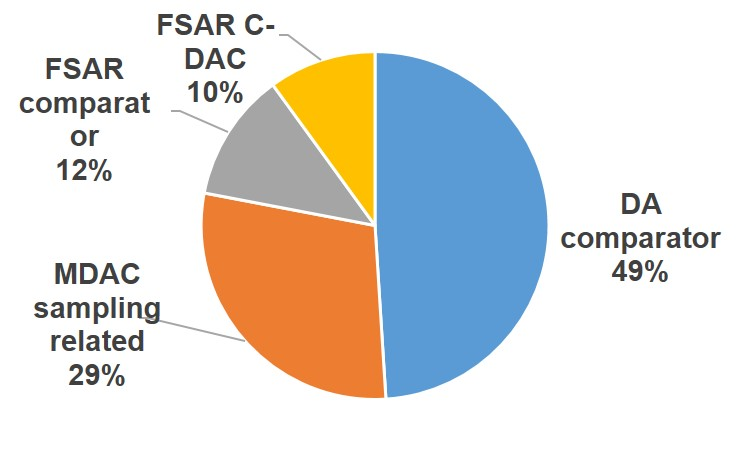
\includegraphics[width=1\textwidth]{figure/chap2/noise-breakdown.jpg}
 \caption{Noise contribution breakdown of the ADC.}
 \label{noise}
\end{figure}

Fig.\ref{noise} shows the noise breakdown of the designed ADC. The 1st stage MDAC consumes about 75\% of the noise, and the majority results from the DA comparator. Therefore, the DA comparator itself must be carefully designed to meet the overall noise requirements. The noise resulting from kT/C and MDAC capacitors ($C_S$ and $C_F$) are rather small because the MDAC capacitor size was chosen for sufficient matching requirements. 

\section{Circuit Implementation}
\subsection{Operational Amplifier}
%%%%%%%%%%%
\begin{figure}[!]
\centering
  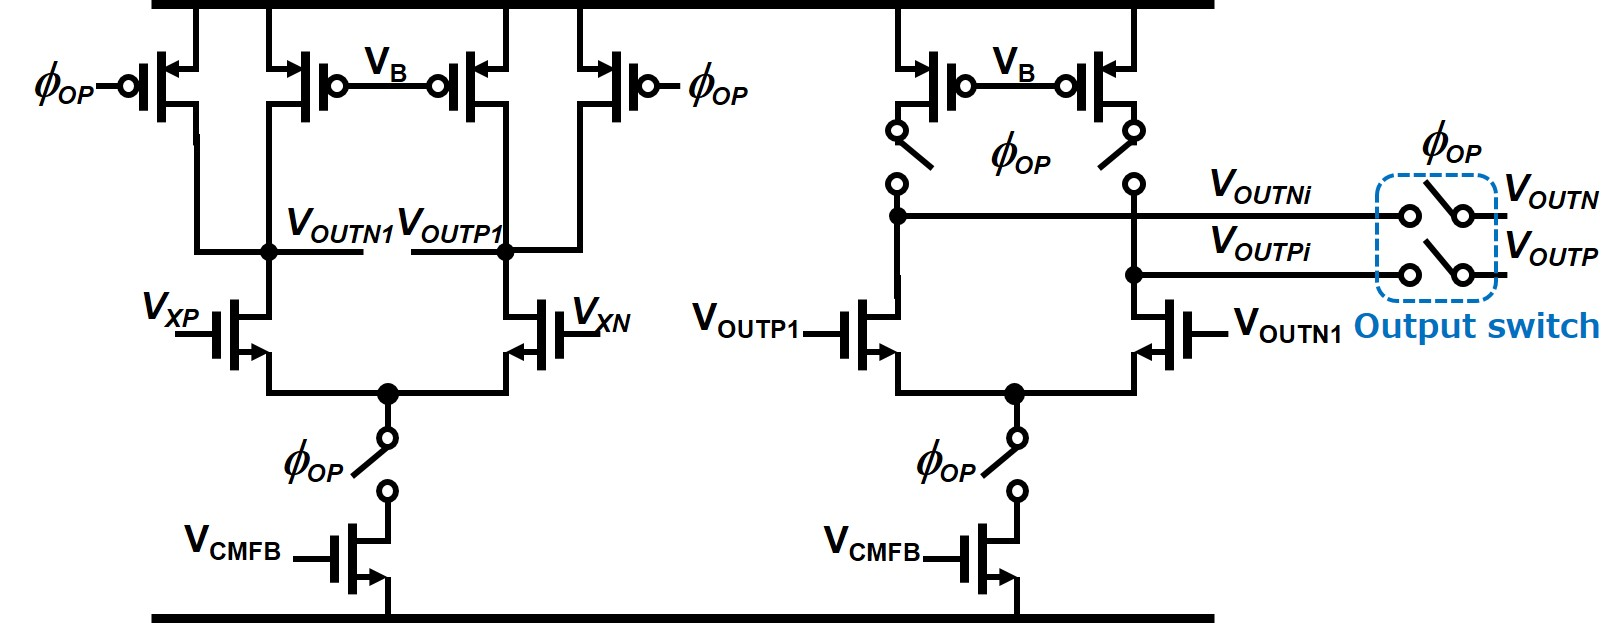
\includegraphics[width=1\textwidth]{figure/chap2/opamp.jpg}
  \caption{Schematic diagram of the designed opamp.}
  \label{fig-opamp}
\end{figure}
\begin{figure}[!]
\centering
  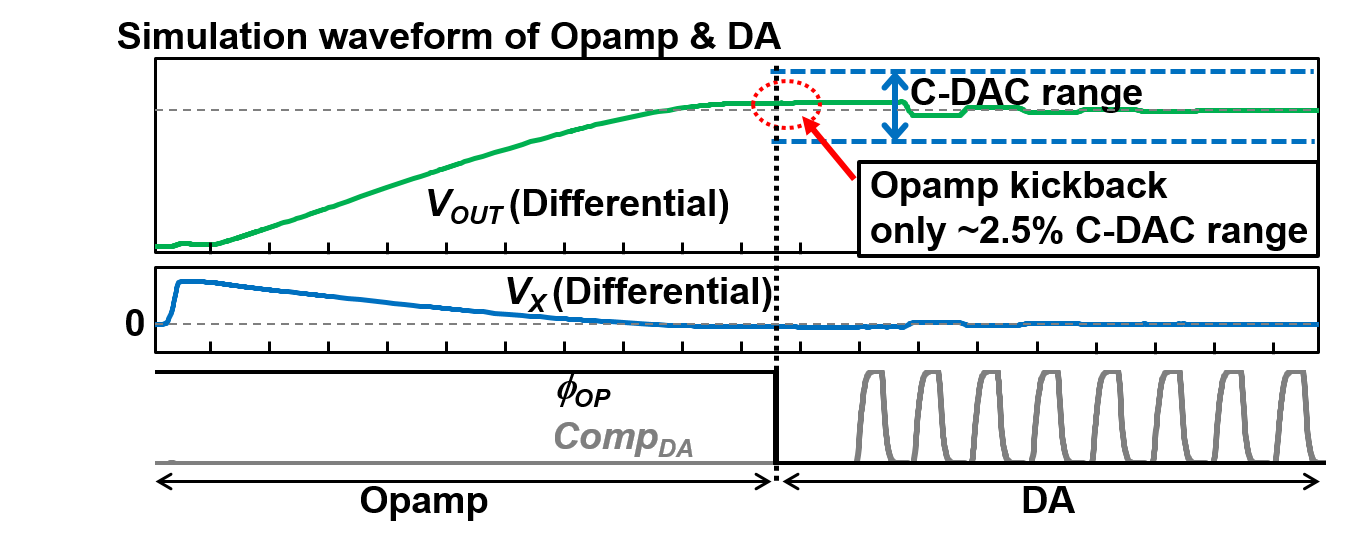
\includegraphics[width=1\textwidth]{figure/chap2/opamp-sim.png}
  \caption{Simulated waveform of the DA-based MDAC. While turning off the opamp causes kickback, the noise is small enough so that it can be canceled by DA operation.}
  \label{fig-opamp-sim}
\end{figure}
%%%%%%%%%%%

The opamp schematic of the designed MDAC is shown in Fig.\ref{fig-opamp}. To accomplish low-voltage operation down to 0.7V, we did not use a cascode and adopted a simple two-stage architecture. While the second stage output drives a large output capacitance load (few pF), the first stage drives only a small load ($<$ 100 fF) with a small gain. To optimize the power consumption of such opamp, we  placed the dominant pole at the second stage output as in ref.\cite{hoDSM2015}, instead of a miller compensation. Pole-splitting is achieved by proper sizing of the first stage so that it will achieve enough $g_m$ and place the 1st stage output pole at high-frequencies. Since settling errors due to instability can also be canceled out by the DA, the phase margin design target is relaxed in our design (40-50$^\circ$).

Also, a power gating scheme is adopted to minimize the opamp power. The opamp only operates during $\phi _{OP} = High$ and does not consume power otherwise; the source current is gated as in ref.\cite{chai20125}. However, since the DA operates in a sample-and-hold fashion as in SAR ADCs, we must design the opamp to minimize the kickback noise during DA operation.
Due to the low off-resistance of scaled CMOS devices, voltage nodes $V_{outP1}$ and $V_{outN1}$ may cause a large drift due to leak currents. Such voltage variation will kickback to $V_x$ (opamp input) through the gate-drain coupling of the input transistor, which will interfere with the DA operation and damage the amplification accuracy.
In order to prevent such problems, the designed opamp resets $V_{outP1}$ and $V_{outN1}$ to $V_{DD}$ after 
$\phi$OP sets down. While this will cause an initial kickback noise when the DA operation starts, its size is less than 2.5\% of the DA C-DAC range and can easily be canceled out (Fig.\ref{fig-opamp-sim}).

\subsection{Comparator Designs}
As we have shown in the last section (Table \ref{noise}), the DA comparator contributes most to the ADC noise performance and must be carefully designed. In our design, to achieve both high-speed and low-powered operation, a two-staged dynamic comparator similar to ref.\cite{miyahara2008low} was adopted. By careful sizing of the input transistors and bandwidth limiting capacitors, the comparator achieves an input-referred-noise of 160$uV_{rms}$ in typical conditions. According to system-level simulations, this comparator noise level requirement is similar to 12-bit SAR ADC with the same input signal voltage ($1V_{pp}$) which is not an excessive requirement. 

Moreover, we found that even with such a low-noise comparator, the power consumption was only 1/3 of the power-gated opamp. Therefore, the power-dominating circuitry is still the opamp (the power breakdown is shown in the measurement section). However, the comparator power will increase exponentially if we target higher resolutions. To mitigate its power, we can adapt low-power techniques such as data-driven comparator\cite{harpe20132}, LSB averaging\cite{moriesaradc} and VCO comparator\cite{yoshiokaVCO} but will prolong the DA amplification time in return. Lastly, we would like to note that the DA comparator offset will appear as the MDAC output offset, similar to an opamp output offset. Since our MDAC has 0.5-bit redundancy, such offset does not affect the ADC performance and we do not calibrate the comparator offset in our design. 

\subsection{DA C-DAC Designs}
%%%%%%%%%%
\begin{table}[!]
\centering
  \caption{The design of the 8-bit DA C-DAC.}
  \label{tbl:Cdac}
 
\includegraphics[width=1\textwidth]{figure/chap2/table-cdac.png}
\end{table}

\begin{figure}[!]
\centering
  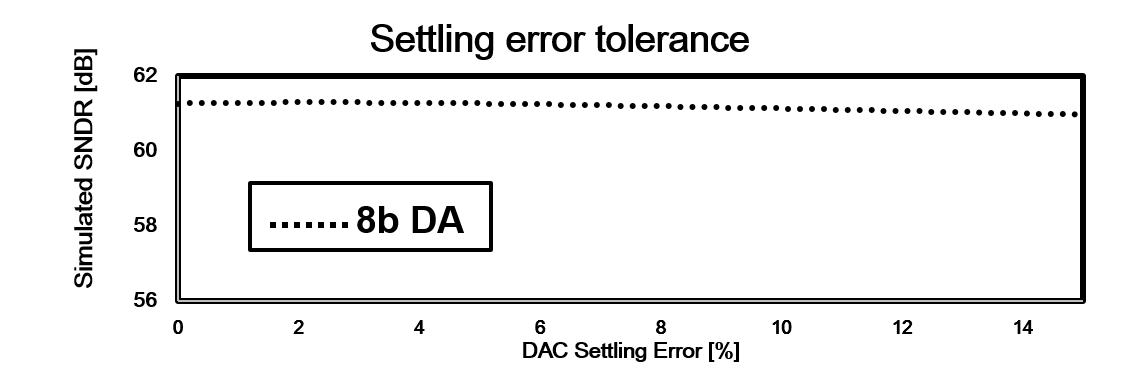
\includegraphics[width=1\textwidth]{figure/chap2/settling-cdac.png}
  \caption{DA C-DAC settling error versus ADC SNDR is shown. Since we utilize redundancy in the DA C-DAC, it is robust to settling errors.}
  \label{fig-cdac-settling}
\end{figure}
%%%%%%%%%%%

\begin{figure}[!]
\centering
  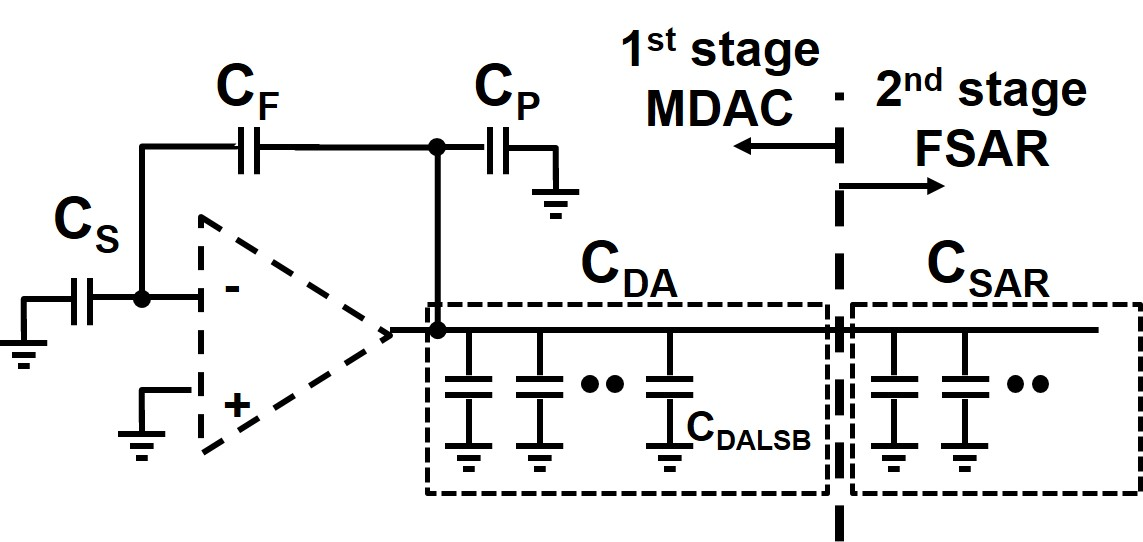
\includegraphics[width=1\textwidth]{figure/chap2/capacitor-network.jpg}
  \caption{Simplified figure of the ADC capacitor network.}
  \label{fig-capacitor-network}
\end{figure}

The structure of the 8-bit (7-bit + 1-bit redundancy) C-DAC utilized in the DA (we will call this DA C-DAC) is shown in Table \ref{tbl:Cdac}. To add settling error resistance to most of the bits, we design the DA C-DAC with 1-bit redundancy and a sub-binary radix of 1.73. The DA C-DAC settling error tolerance was simulated in Fig.\ref{fig-cdac-settling}. Even with a settling error of 15\% in every bit, the SNDR degradation is only $<$ 1dB. While this 1-bit redundancy can relax the reference voltage designs significantly, the DA amplification time prolongs for 14\% due to extra cycles.

% どうやってオペアンプのmaxエラーを導出するかについて記述する。設計フローについて記述。
As discussed in the previous sections, the absolute value of $V_{CDACLSB}$ directly couples to the DA accuracy and must be carefully designed. Here,  we will discuss the C-DAC design methods to meet the target of $V_{CDACLSB}$. According to system simulations, the $V_{CDACLSB}$ must be designed to be bellow 1.6mVp to accomplish the target amplification accuracy. Importantly, $V_{CDACLSB}$ is decided by the ratio between the DA C-DAC LSB capacitor ($C_{DALSB}$) and the total load capacitance seen at the amplifier output. Fig.\ref{fig-capacitor-network} shows the simplified capacitor network. The main load capacitors are the total capacitance of DA C-DAC $C_{DA}$, the total capacitance of FSAR C-DAC $C_{SAR}$, feedback capacitor seen from the MDAC output $C_F$ and parasitic capacitance $C_p$. 

$V_{CDACLSB}$ can be derived via capacitive dividing as bellow.
 \begin{equation}
    V_{CDALSB} =V_{ref} \times \frac{C_{DALSB}}{C_{DA}+C_{SAR}+C_P+C_{S+F}}  
 \end{equation}
Here, the serial capacitance of $C_S$ and $C_F$ is shown as $C_{S+F}$ and $V_{ref}$ is the reference voltage of the C-DAC. Since the parasitic $C_P$ relies heavily on the layout, several iteration of layout-parasitic-extraction (LPE) was  required to fix the value of $C_{DALSB}$. After LPE simulations, we fixed the $C_{DALSB}$ to 2.4fF to meet the target $V_{CDACLSB}$.


\section{Measurement Results}
\begin{figure}[!]
\centering
  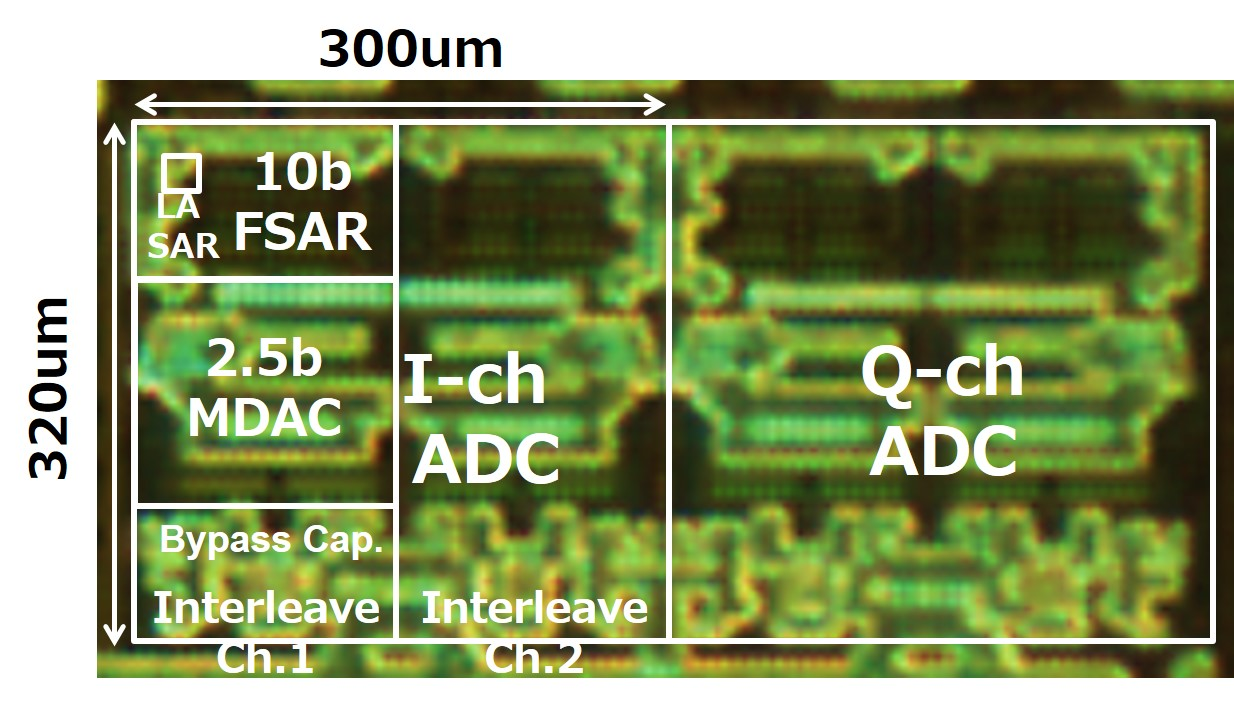
\includegraphics[width=0.8\textwidth]{figure/chap2/chip.jpg}
  \caption{Chip photo of the prototype ADC. Evaluation results of the I-channel ADC are shown. }
  \label{fig-chip-photo}
\end{figure}
%%%%%
\begin{figure}[!]
\centering
  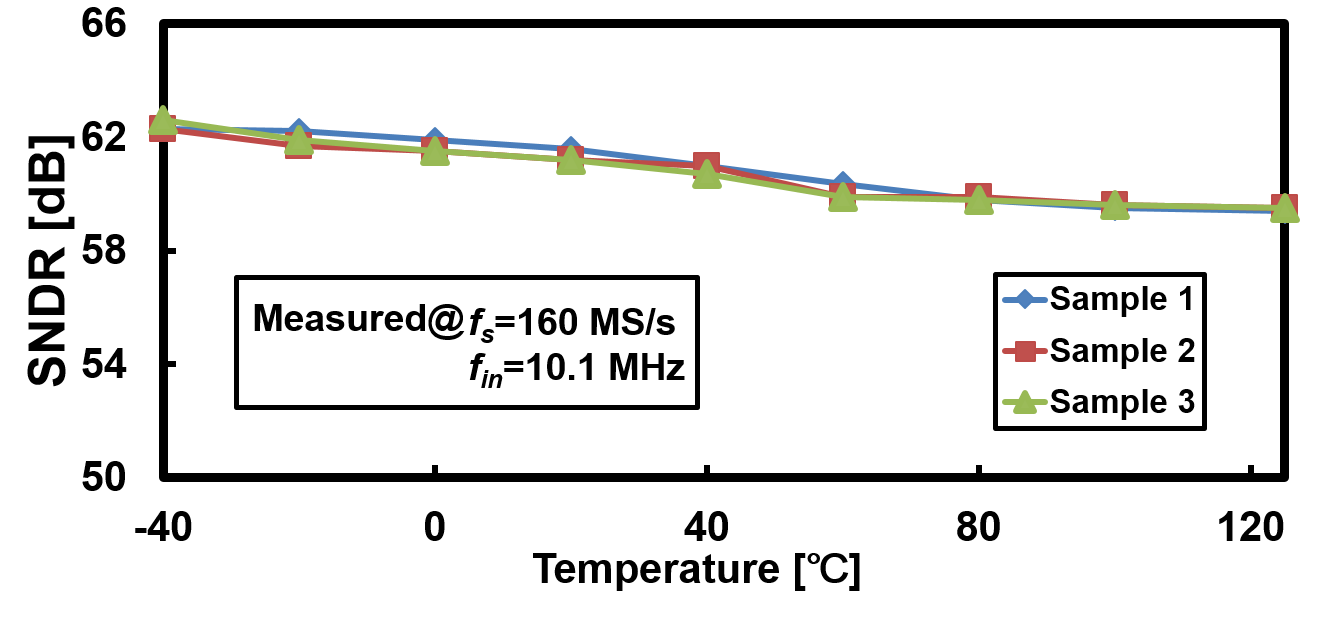
\includegraphics[width=1\textwidth]{figure/chap2/meas-thermal.png}
  \caption{ADC measured performance from 3 randomly selected chips. Temperature vs ADC SNDR were measured.}
  \label{fig-meas-thermal}
\end{figure}
%%%%%
\begin{figure}[!]
\centering
  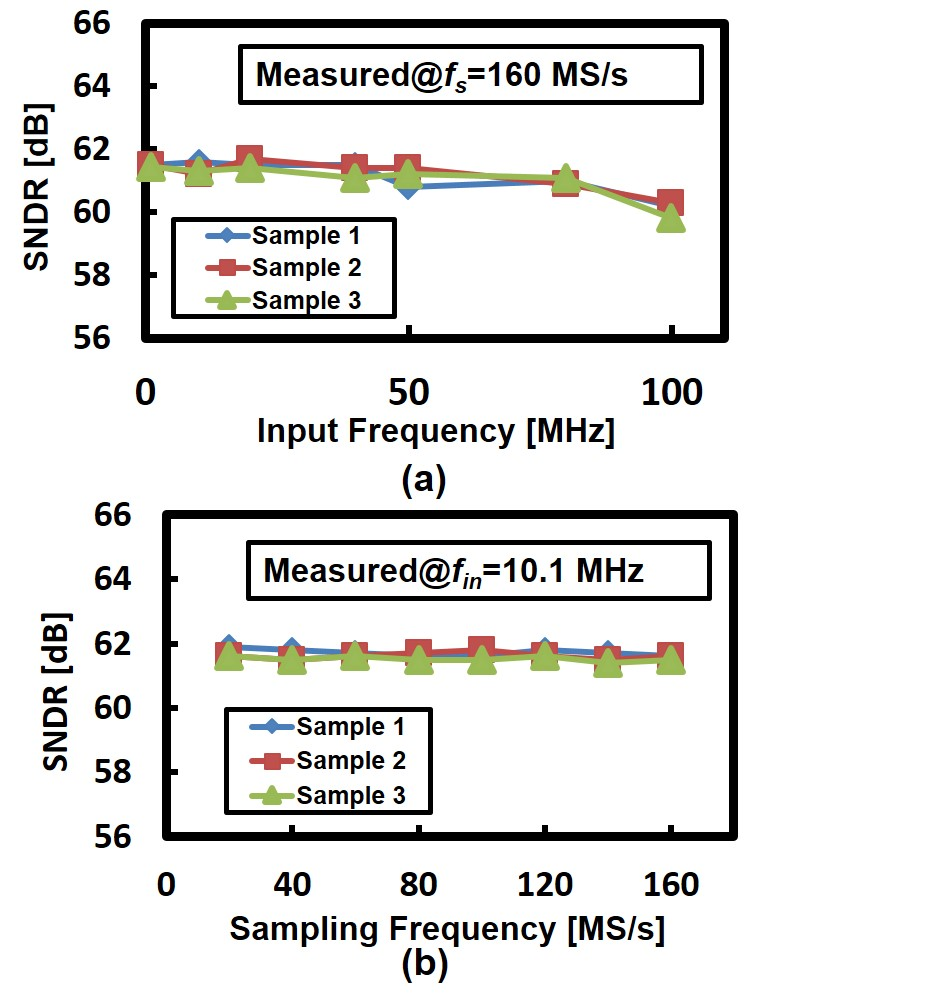
\includegraphics[width=1\textwidth]{figure/chap2/meas-input-fs.jpg}
  \caption{ADC measured performance from 3 randomly selected chips. (a) Measurement with varied $f_s$ (b) Measurement with varied $f_{in}$.}
  \label{fig-meas-input-fs}
\end{figure}
%%%%%
\begin{figure}[!]
\centering
  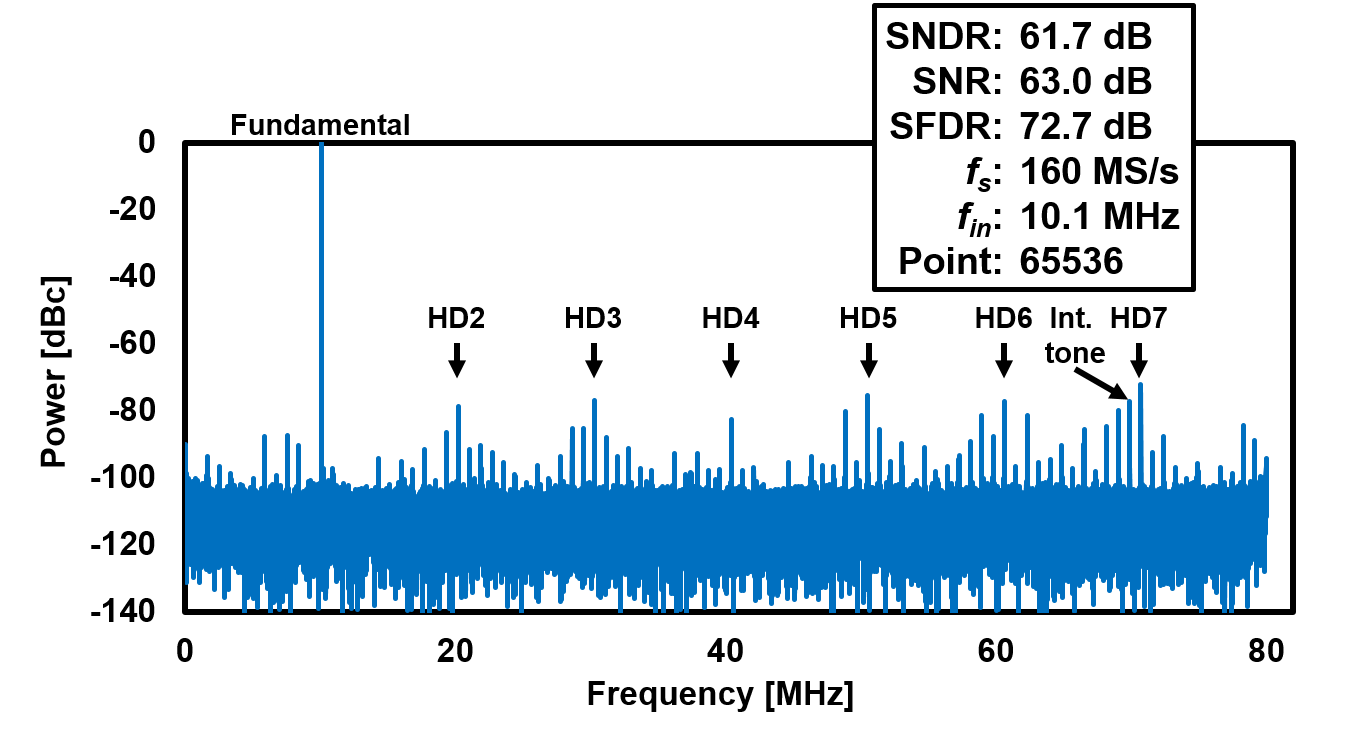
\includegraphics[width=1\textwidth]{figure/chap2/FFT.png}
  \caption{ADC FFT measured results at $f_{in}$=10.1 MHz.}
  \label{fig-FFT}
\end{figure}
%%%%%
\begin{figure}[!]
\centering
  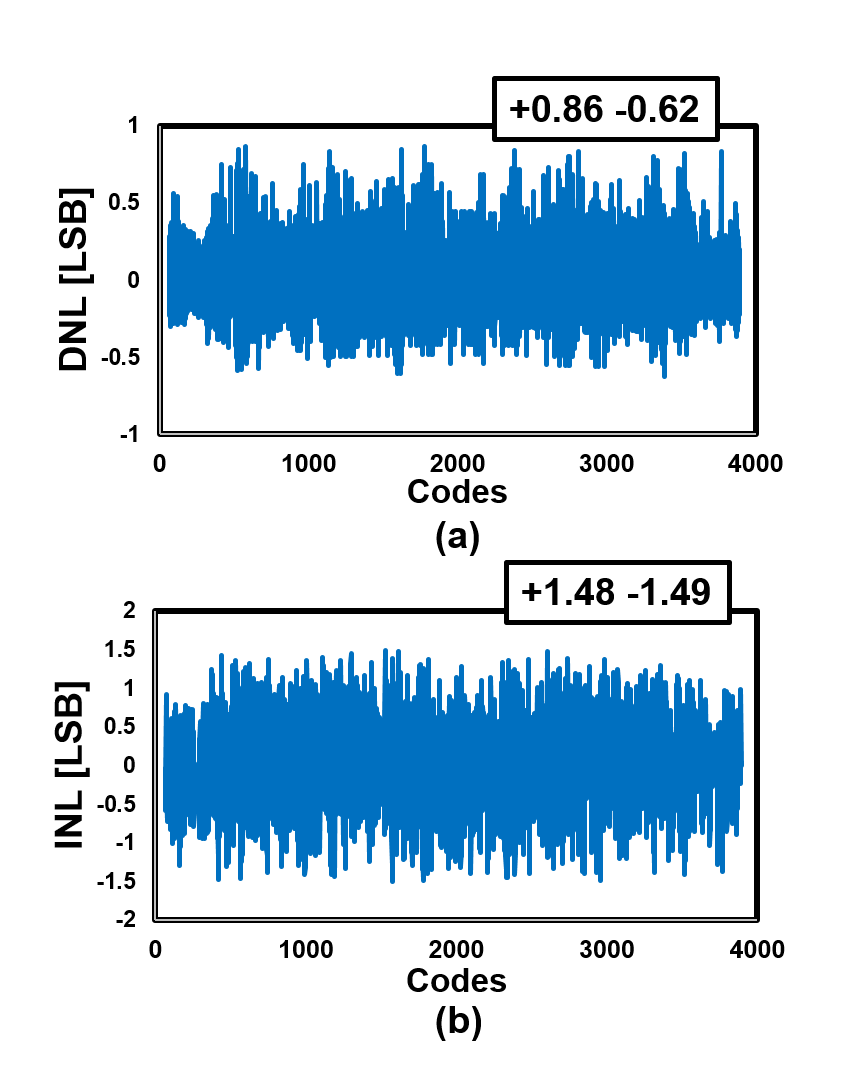
\includegraphics[width=0.7\textwidth]{figure/chap2/dnl-inl.png}
  \caption{(a) ADC measured DNL. (b) ADC measured INL.  }
  \label{fig-DNL}
\end{figure}
%%%%%


The ADC implemented in 28nm CMOS consumes 0.097mm$^\text{2}$, which also includes 70pF bypass capacitor for the ADC reference voltage (Fig.\ref{fig-chip-photo}). Owing to DA’s robustness and efficient use of DA C-DAC's redundancy, a low-cost implementation was accomplished. At typical conditions, the ADC achieves SNDR of 61.1dB with 160MS/s Nyquist input and the power consumption is only 1.9mW. The power includes all necessary ADC components: clock buffer, error correction, reference voltage, and current reference generation. The corresponding walden-FoM is 12.8fJ/conv. To emphasize the calibration-free feature of the DA-based pipelined ADC, we did not apply any calibration for the reported measurement results. However, the effect of inter-channel offset is not included in our measurements, and the reason is described later.


To maximize the power-efficiency, the main measurements were carried out with a power supply voltage of 0.7V. The ADC speed can be significantly improved by turning the supply up to 0.9V; 320MS/s can be achieved with a slightly worsened SNDR of 59.6dB. In our measurements, we fixed the input swing to 1Vpp and the SNR performance is similar for both supply voltages. The SNDR is slightly lower for 0.9V because of higher input frequency (160MHz), which poses higher distortions in the sampling. However, the power-efficiency greatly degrades to 32.1fJ/conv. because the opamp draws a larger current for high-speed operation and the digital circuit power increases with higher supply voltages.

Fig.\ref{fig-meas-thermal} shows the temperature variation versus ADC SNDR characteristics of 3 randomly chosen samples.  To confirm the calibration-free ADC’s robustness, the temperature variation of -40 to 125$^\circ $C was applied, and all samples achieve SNDR$>$59.5dB with 160MS/s operation.  At a high temperature, the comparator noise of DA limits the SNDR. As the temperature goes down, the thermal noise decreases and SNDR is pushed up.  Moreover, the SNDR is well flat with varied $f_s$ and $f_{in}$ (Fig.\ref{fig-meas-input-fs}).

Fig.\ref{fig-FFT} shows the FFT spectrum of the ADC. As analyzed in Section IV, the DA is fundamentally spurious-free but SFDR was limited to 73dB in measurements. With further analysis, we found that the MDAC layout induced capacitor mismatches limit the SFDR. The spurious tones appeared in all of the measured samples similarly regardless of PVT variations. Furthermore, simulations showed that the SFDR can be further improved either by capacitor rotating or with digital gain calibration. The ADC DNL/INL measured results are reported in Fig.\ref{fig-DNL}.

\begin{figure}[!]
\centering
  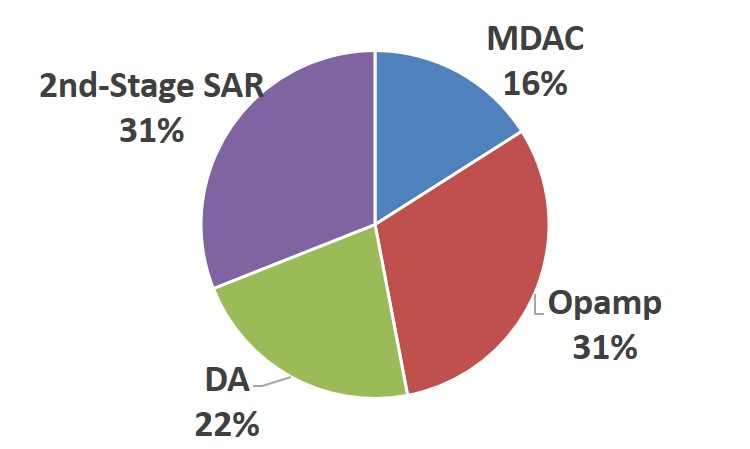
\includegraphics[width=1\textwidth]{figure/chap2/power-breakdown.jpg}
  \caption{Simulated power breakdown of the ADC.}
  \label{fig-power-breakdown}
\end{figure}


In 2-channel time-interleaved ADCs, the inter-channel offset mismatch effects appear at the DC and Nyquist Frequency.  However, in our measurements, we calculate the FFT and SNDR by removing the DC and Nyquist Frequency bin; the inter-channel offset mismatch effect is excluded in our design.
Generally, wireless baseband ADCs are utilized with an oversampled situation and useful information rarely exists at the Nyquist Frequency and can be removed without impacting the wireless system performance.
In cases where the Nyquist Frequency is of interest, inter-channel offset calibrations should be implemented to suppress the offset mismatch effects. Offset calibrations are less complex compared to gain calibrations and will have little impact on the start-up time. By suppressing the Nyquist tone down to SFDR $<$ 75dB, the ADC SNDR will not be affected. For such cases, the inter-channel relative offset should be $<=$ 2 LSB which can be easily realized by digital calibrations.

Fig.\ref{fig-power-breakdown} shows the simulated power breakdown of the ADC. The 1st stage MDAC consumes almost 70\% of the entire energy and rest is the 2nd stage SAR. Still, the opamp is the dominates the power consumption, since it must complete a coarse but fast amplification. Future research may be pointed to making the coarse amplifier power-efficient; ring amplifiers \cite{hershberg2012ring} and dynamic amplifiers \cite{verbruggen20132} will be a great fit for such roles.


\subsection{Scaling Effects of the Digital Amplifier}
%%%%%%
\begin{figure}[!]
\centering
  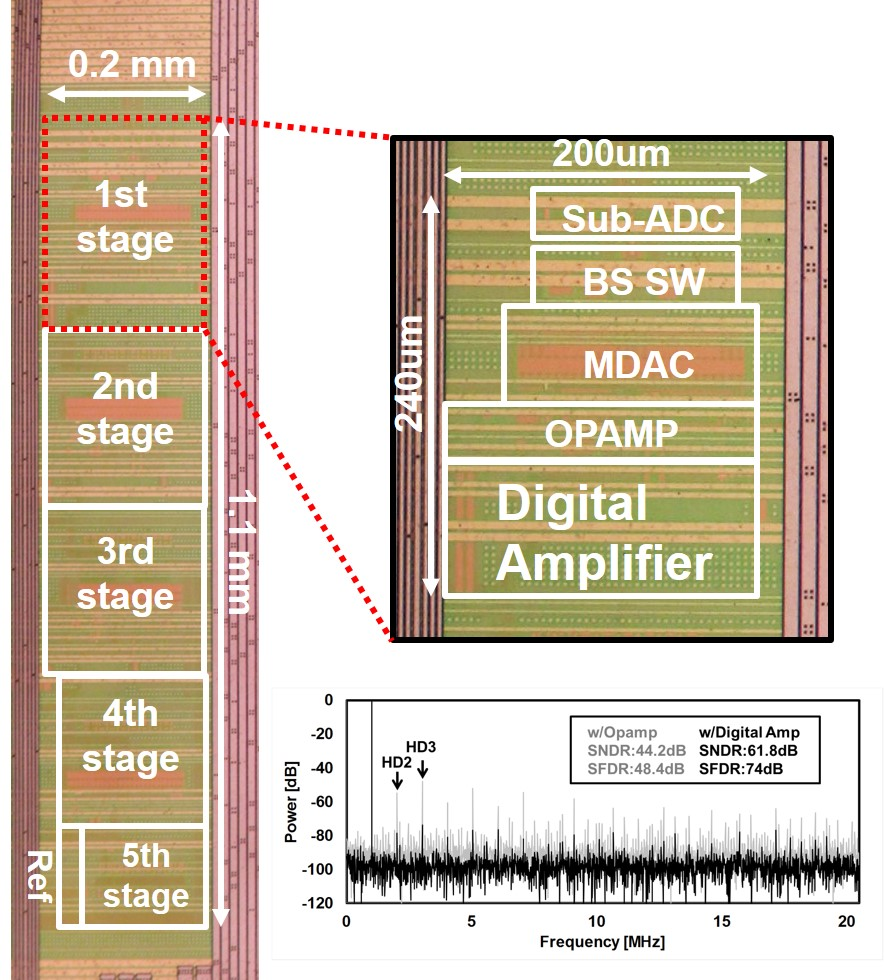
\includegraphics[width=0.8\textwidth]{figure/chap2/65nmchip.jpg}
  \caption{A digital amplifier-based 11-bit pipelined ADC prototyped in 65nm CMOS.}
  \label{fig-65nm}
\end{figure}
%%%%%
\begin{table}[!]
\centering
  \caption{Inter-process comparison of the digital amplifier-based MDAC. }
  \label{tbl:process}
 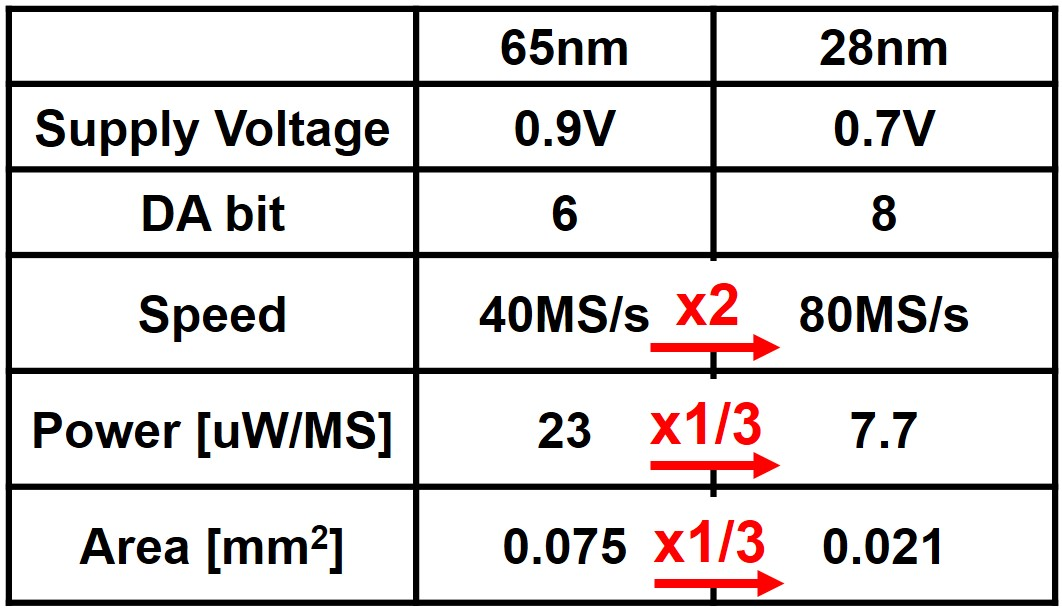
\includegraphics[width=0.8\textwidth]{figure/chap2/performancecomp.jpg}
\end{table}
%%%%%
\begin{table*}[!]
\centering
  \caption{Performance Comparison with state-of-the-art Pipelined and Pipelined-SAR ADCs.}
  \label{tbl:performancecomp}
 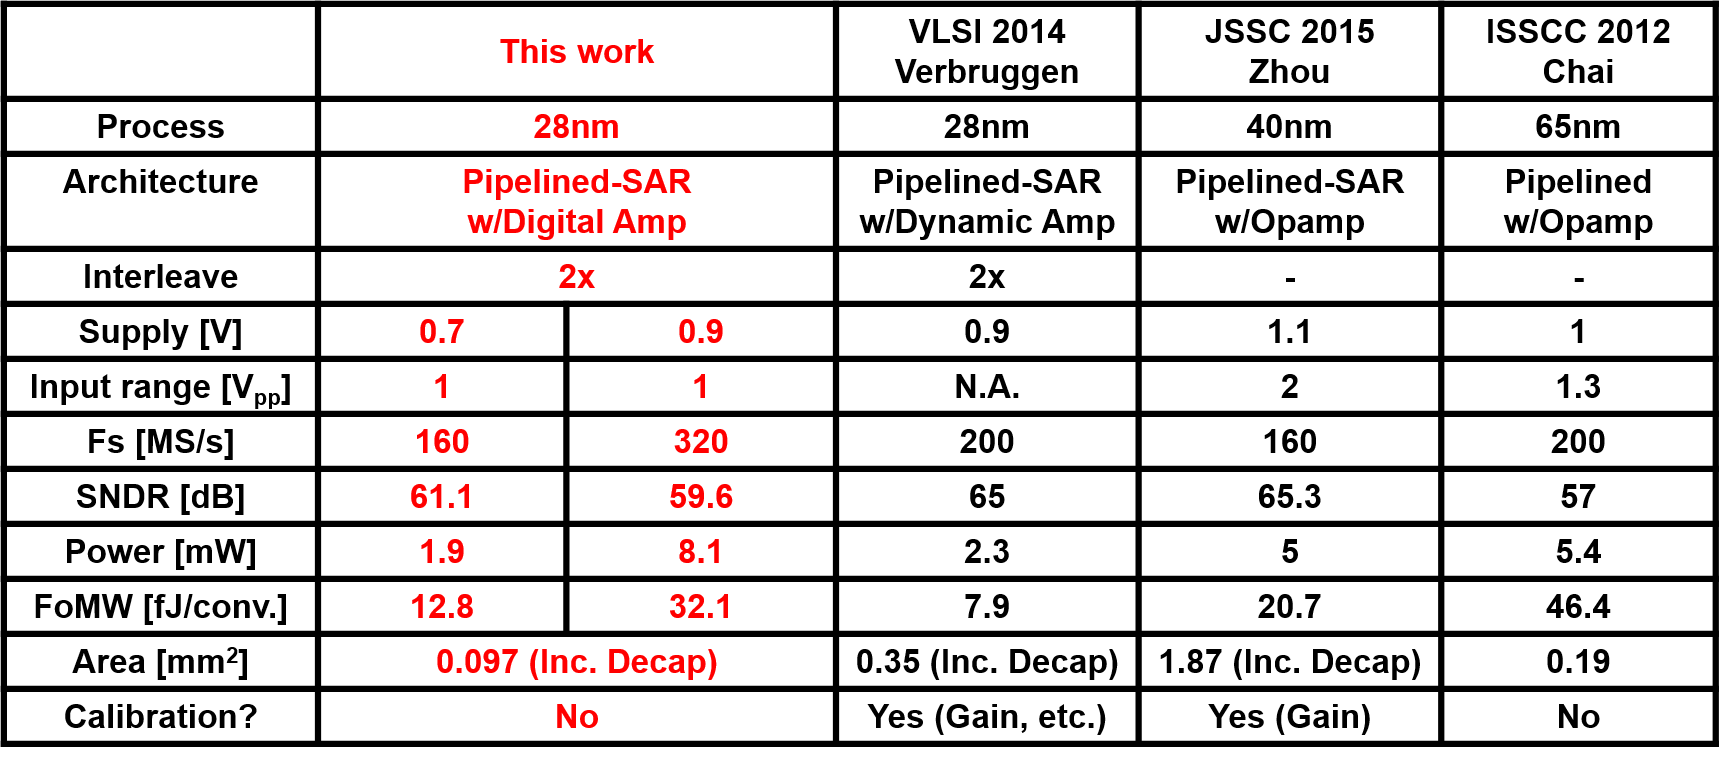
\includegraphics[width=1\textwidth]{figure/chap2/performancecomp.png}
\end{table*}
%%%%%
In order to evaluate the process scaling effects of the digital amplifier, an adequate approach is to implement the same circuit in different CMOS process and compare the performance.
Therefore, to conduct an inter-process evaluation of the DA, we prototyped a DA-based 12-bit pipelined ADC in 65nm CMOS (Fig.\ref{fig-65nm}). The ADC is designed with a similar noise budget and accomplishes an identical SNDR of 61.8dB. Importantly, the DA's core circuit is identical, sharing the design of the comparator and the SA logic. While the ADC architecture differs (Pipelined and Pipelined-SAR) and a direct comparison cannot be made, the 1st MDAC stage designs are almost the same and will be employed to evaluate the DA's process scaling effects.

Table \ref{tbl:process} compares the performance of the 1st MDAC stages. Since better opamp gain performance can be achieved with 65nm CMOS, its DA is designed with 6-bit. However, the DA cycle speed greatly outperforms in 28nm CMOS and achieves 2$\times$ speed improvements. Moreover, the DA area and power efficiency were significantly enhanced with 28nm CMOS due to the digital nature of the DA and 3$\times$ improvement were observed. The power-efficiency is also benefited from using low supply voltage (0.7V) in 28nm CMOS. We expect a continuous performance improvement of the DA-based MDACs with further scaled processes, as long as the digital circuit keeps improving its performance. 

\subsection{Benchmarks}

\begin{figure}[!]
\centering
  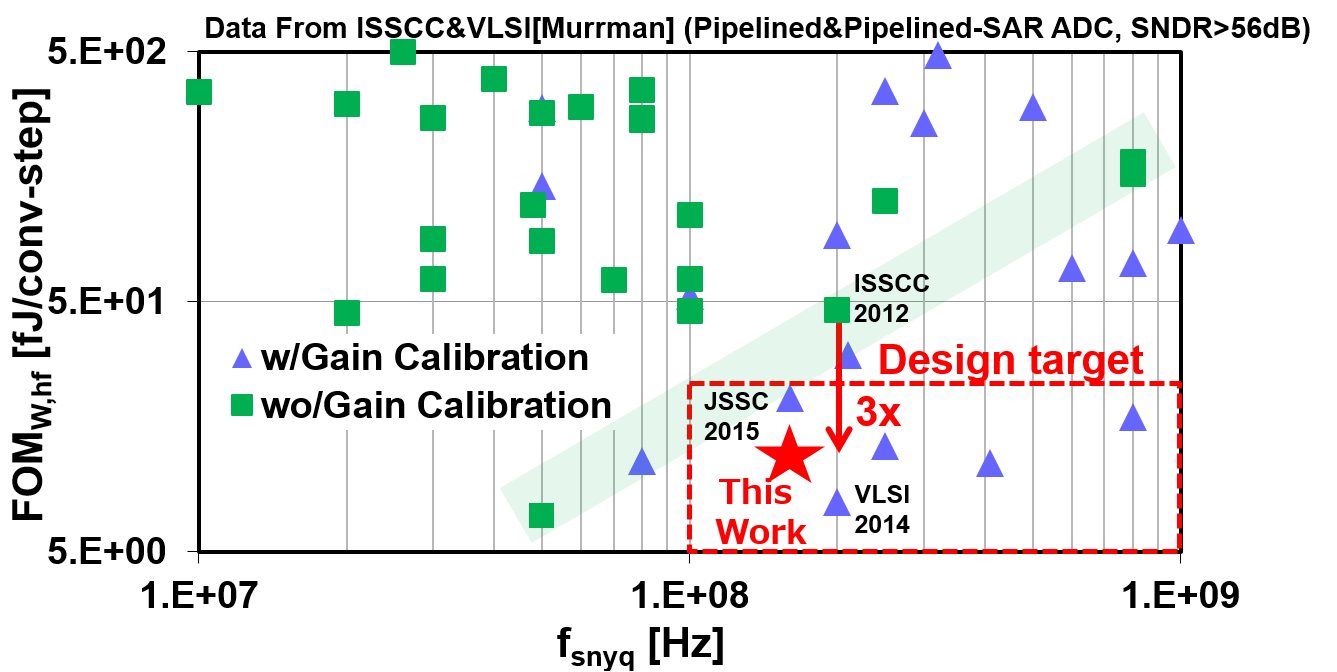
\includegraphics[width=1\textwidth]{figure/chap2/bench.png}
  \caption{Benchmark against Pipelined and Pipelined-SAR ADC published in ISSCC and VLSI. Our work achieves 3$\times$ power efficiency improvement compared to ADCs without gain calibrations.}
  \label{fig-bench}
\end{figure}
%%%%%
Table \ref{tbl:performancecomp} compares our ADC performance against state-of-the-art pipelined-SAR and pipelined ADCs achieving similar performance \cite{verbruggen201470}, \cite{zhou201512}, \cite{chai20125}. While accomplishing a competitive energy efficiency to pipelined ADCs utilizing open-loop amplifiers and gain-calibration, our ADC did not require any calibration at all. Moreover, the required overall ADC area is $3-18\times$ smaller. While prior works with open-loop amplifiers utilize bypass capacitors of several nF due to low power supply rejection, DA is robust to power supply noise and our work design only uses 70pF capacitors for decoupling. 

Moreover, based on \cite{MurmanADC}, the author categorized either the ADC utilize gain calibration or not to perform an extensive comparison between works published in ISSCC and VLSI (Fig.\ref{fig-bench}). ADCs meeting our design target ($fs>$100MS/s, FoM$<$20fJ/conv., SNDR$>$56dB) conventionally employed gain-calibration, which had underlying issues on SoC start-up time and stability. For the author's best knowledge, our ADC achieves FoM of 12.8fJ/conv. without calibration, which is a 3x improvement compared to the conventional calibration-free pipelined and pipelined-SAR ADCs with $fs>$50MS/s and SNDR$>$56dB. 

\section{Conclusions}
We introduced the concept and implementation of the digital amplifier (DA) to realize a calibration-free, process scaling pipelined-SAR ADC. 
The amplification features of the DA were extensively studied, such as the gain-error principles and spurious-free characteristics. We showed that the DA accuracy is determined by the C-DAC LSB step and irrelevant to intrinsic gain, showing potential for further process scalability. In addition, due to the relaxed settling requirements, we showed that significant power savings can be achieved compared to opamp-based MDACs.

Measurement results of the calibration-free 0.7V 12b 160MS/s pipelined-SAR ADC were reported. Without any calibration, the ADC achieved SNDR=61.1dB, FoM= 12.8fJ/conv., archiving over 3x power efficiency improvement compared to conventional calibration-free high-speed pipelined ADCs. Finally, an inter-process performance comparison was executed to confirm the process scalability of the DA.

